\documentclass{article}
\usepackage{iclr2025_conference,times}
\input{math_commands.tex}

\usepackage{amsmath,amssymb, comment}
\usepackage{graphicx}
\usepackage{float}
\usepackage{xcolor}
\usepackage{url}
\bibliographystyle{unsrtnat}

\iclrfinalcopy          % non-anonymous (shows authors); comment out for anonymous submission

% gray-italic scaffolding note: what should go in a section
\newcommand{\scaffold}[1]{{\par\color{gray}\itshape #1\par\medskip}}

% placeholder box for figures still to be generated
\newcommand{\figplaceholder}[2][0.6\linewidth]{%
  \fcolorbox{gray}{gray!8}{\parbox[c][3.2cm][c]{#1}{\centering\ttfamily\footnotesize
  \textcolor{red}{[GENERATE]}\\[2pt] #2}}}

\title{AlloBench: Measuring Online Tool Allocation Capability in LLM Agents}

\author{%
Daniel Wang\thanks{These authors contributed equally to this paper.} \quad
Andrew Xu\footnotemark[1]\\
Sea12 Technologies \quad Yale University \\
\texttt{daniel.wang.dzw22@yale.edu}}

\newcommand{\fix}{\marginpar{FIX}}
\newcommand{\new}{\marginpar{NEW}}

\begin{document}
\maketitle
\begin{abstract}
Creating a reusable tool is an investment: an agent pays a fixed cost now in
exchange for the potential of future reuse. Therefore, a user should prefer an agent that creates a small number of highly reusable tools, rather than many one-offs. We introduce a paired, scored benchmark that tests whether LLM agents exhibit conscious allocation behavior under a fixed budget in two contexts: an abstract text-based formulation and a code-construction task. We find that every frontier model we test -- Claude Haiku, Claude Opus, GPT-5.4-mini, and GPT-5.6 Sol -- acts near-optimally in the abstract framing but fails to transfer this ability to script-writing. Through further experiments, we
identify the particular failure modes for each model. Notably, the first three models fail even when the scripts are not evaluated, while GPT-5.6 Sol stays selective under that weaker manipulation and collapses only at full construction -- evidence that the code-required task is passable and the shared failure marks a genuine capability boundary rather than an impossible task.
Furthermore, a Qwen2.5-Coder-14B model policy-trained for abstract allocation generalizes this ability across held-out lexical
variations, but sees minimal improvement at script allocation.
Together, these results establish online tool allocation as a significant
capability boundary, even for modern frontier models.
\end{abstract}

\section{Introduction}

Large language model (LLM) agents are increasingly used to create scripts, wrappers, macros, and skills that can be reused across tasks. Existing evaluations ask whether a model can
write a correct tool, choose an available tool, or select from a growing
library \citep{cai2024latm,qian2023creator,huang2024ultratool,qu2025toollearningsurvey}. 
They largely leave a more fundamental decision unmeasured: \emph{when} should the agent create a tool? 

Building tools---API calls, Python scripts, or video game macros---is expensive, consuming both time and tokens. For individual tasks, paying this cost is almost always either obviously worthwhile or clearly unnecessary. On the other hand, agents that may expect to see certain tasks recur often must take this tradeoff more seriously: tool creation pays a fixed cost but makes future uses far cheaper. An agent facing an unknown task stream therefore has two
options at each turn: build a script for the current task or wait for more evidence of recurrence. Building too eagerly wastes resources on rare tasks that could have been better treated by hand; waiting too long forfeits useful reuse. 

The cost of tool construction is difficult to pinpoint. For example, the number of tokens needed for a model to generate a Python script depends on the capability of the model and the complexity of the task. This leaves providers of agentic services in a difficult position---in principle, the model itself should decide when building is beneficial, but recent work has shown that current models fail to do so reliably \citep{lin2026bagen}. An alternative approach to encourage more prudent tool usage is to present the agent with a limited action budget \citep{liu2025budgetaware}. One might hope and suspect that decreasing the number of scripts an agent is permitted to write over a stream of tasks would make it more selective with its tool creation. We show in this paper that this fails to hold, even in the most capable of modern frontier models.

A small but growing set of studies---many from the last year---have analyzed how LLM agents respond to budget awareness. A consensus seems to be that models are naturally poor at budgeting, but that this capability can be easily post-trained through a variety of techniques \citep{liu2025budgetaware, lin2026bagen, li2026bavt, ding2026calibrate}. We find this assessment only partially accurate. By introducing a paired benchmark to test budget-aware tool investment, we find that a significant capability wall exists at the gap between abstract allocation and tool creation, which has not yet been addressed in a budget-aware context. Furthermore, knowledge gained from the former does not transfer to the latter, revealing a fundamental and unexpected failure mode in modern LLMs. 

In this paper, we use an experimental structure that intentionally generalizes to a variety of domains. In one session, we present the agent with a sequence of $N$ tasks chosen from a hidden distribution. The agent can create at most $T$ tools throughout the entire session, and tools can be reused once made. Because tasks and tools can take any form, this framework can be applied to a wide range of settings; we consider an abstract ball-collection game and a concrete math test. This is an online learning problem, where optimal behavior involves the agent basing its actions based on the already-observed distribution.

Our primary contributions are as follows:
\begin{enumerate}
    \item a generalizable paired benchmark to study budget-aware tool investment, which we call AlloBench;
    \item an accompanying numerical score to fairly compare performance across models;
    \item strong cross-family evidence that frontier models can abstractly allocate budget but fail to do so in tool creation;
    \item an exact identification of the trigger, which sits at required code emission for three of the four frontier models and at full script construction for the strongest;
    \item a small experiment disproving the potential counterpoint that tool allocation fails only because the economics are uncertain;
    \item a demonstration that post-training on abstract budget allocation can fail to transfer to tool creation.
\end{enumerate}

\section{Related Work}

\paragraph{Tool use benchmarks.} LLM tool creation has been evaluated in many varied contexts. The first dataset introduced in this direction was the Creation Challenge \citep{qian2023creator}, which prompts models to write Python scripts to solve algebra word problems. Later benchmarks have primarily focused on simulating realistic settings \citep{huang2024ultratool, yu2026wildtoolbench}. These benchmarks test tool creation, use, and reuse over lengthy problem streams. Numerous methodologies have also been introduced to improve LLM tool capabilities. LATM uses a larger model to write scripts and a smaller model to reuse them
\citep{cai2024latm}; other works such as ReGAL, LILO, and TroVE all induce expandable skill libraries and show improvements over one-shot tool creation \citep{stengeleskin2024regal,grand2024lilo,wang2024trove}. These systems assume that the recurring task warrants construction. In fact, recent work shows that these methods result in much less reuse than expected, instead improving self-correction
\citep{berlotattwell2024librarylearning}. Therefore, an important and necessary question to answer before focusing on inducing reuse is whether LLMs can accurately identify opportunities to apply it.

\paragraph{Budget awareness.} A separate and very recent line of work asks whether agents respond to a fixed budget (primarily of tool calls) at inference time. Budget-Aware Tool-Use finds that granting a larger tool-call budget does not improve web-search agents because they lack native budget awareness \citep{liu2025budgetaware}. The same paper introduces a prompt-level budget tracker and a
budget-aware framework that improves cost efficiency \citep{liu2025budgetaware}. BAGEN evaluates whether agents can estimate  their own remaining budget mid-episode, finding that strong task
performance and capable budget-awareness are only weakly correlated, and even frontier models are over-optimistic \citep{lin2026bagen}. Several other methodologies of increasing budget awareness involve computing the expected utility gain from calling a tool \citep{liu2026utility}, pruning a reasoning tree \citep{li2026bavt}, and planning to maximize the probability of finishing within a deadline and under budget \citep{wang2026mcpp}. This last work studies ``online resource allocation'' by allowing models to allocate compute across
subtasks of a single workflow. Though the terminology is very similar to this paper, it studies a very different problem from tool investment. Notably, none of these studies provide a quantitative metric for budget allocation, and none provide cross-model comparisons. By discretizing the action space with a defined problem stream, we isolate a capability wall for budget-awareness.

\paragraph{Online learning and regret.} From a theoretical standpoint, AlloBench best aligns with prior work on online learning capability in LLMs. We draw inspiration from the theory of LLM \textit{regret} \citep{park2025regret}, which measures the expected reward the agent failed to obtain. LLMs are known to have non-zero regret, even on simple tasks \citep{park2025regret}. Regret has been used as an unsupervised training loss, a method that is proven in theory to improve LLM performance \citep{park2025regret}. In this paper, we employ regret as a post-training loss in reinforcement learning (RL). Our results agree with studies that have demonstrated suboptimal behavior stemming from premature commitment to a strategy \citep{chen2025greedy, mehta2026commit}. The recently-introduced Calibrate-Then-Act framework seeks to prevent this by explicitly providing the agent with an estimated prior about its environment state \citep{ding2026calibrate}.  Separately, small variations in problem structure (e.g. arithmetic in base 9 vs. base 10) have been shown to significantly degrade LLM performance \citep{wu2024counterfactual}. We present the first benchmark designed to test online budget allocation, as well as the first framing gap for online learning.

\section{AlloBench}
\label{sec:allobench}

AlloBench casts reusable tool creation as an online investment decision and
measures it with a paired benchmark: the same latent allocation problem
presented in an abstract frame and a code-construction frame. This section
defines the decision process, how we instantiate and score it, the
experimental protocol under which we run it, and the preregistered framing
ladder we use to localize where behavior shifts between frames.

\subsection{Decision process}

An episode contains a horizon of $T$ items with latent classes
$c_t \in \{1,\ldots,N\}$. At time $t$, the agent observes the current item and
history $h_t$, has remaining build budget $b_t$, and chooses whether to commit
to class $c_t$. A commitment is irreversible and consumes one of $B$ available
builds. Once a class has been built, later occurrences can reuse its artifact.
The class frequencies are unknown at the start of the episode.

For the economic experiments, a solved or collected occurrence contributes
one point and a commitment costs $K$. For policy $\pi$,
\begin{equation}
U(\pi) =
\sum_{t=1}^{T} r_t(\pi)
- K\sum_{c=1}^{N}\mathbb{I}\{\pi\text{ commits to }c\},
\end{equation}
subject to at most $B$ commitments. The best action depends on both recurrence
evidence and remaining budget. A one-off class should not consume a build;
a sufficiently frequent class should.

\subsection{Benchmark construction}
\label{sec:construction}

We instantiate the process with streams of $T=60$ numeric problems drawn from
eight latent problem families. Each canonical stream contains approximately
three ``hot'' classes that recur 13--23 times and several ``trap'' classes that
appear only 1--6 times. An early-trap constraint places a rare class among the
first $B$ opportunities, making first-sight commitment costly. The hardened
numeric pool is designed to make unaided hand solving approximately unavailable
while retaining script-based solvability.

The abstract and constructive environments are views of the same latent class
sequence. In the abstract urn frame, the model observes a colored item and
chooses \textsc{keep} or \textsc{pass}. Keeping a class commits budget and
collects its occurrences. In the reusable-script frame, the model encounters a
numeric problem and may write a class-level solver that can be run on later
instances. We pair identical latent class identities, roles, counts, and arrival
orders across conditions. Numeric payloads may be rendered at a model-calibrated
magnitude without changing that latent sequence.
Figure~\ref{fig:frames} illustrates this isomorphism on the opening turns of a
single canonical stream.

\begin{figure}[t]
\centering
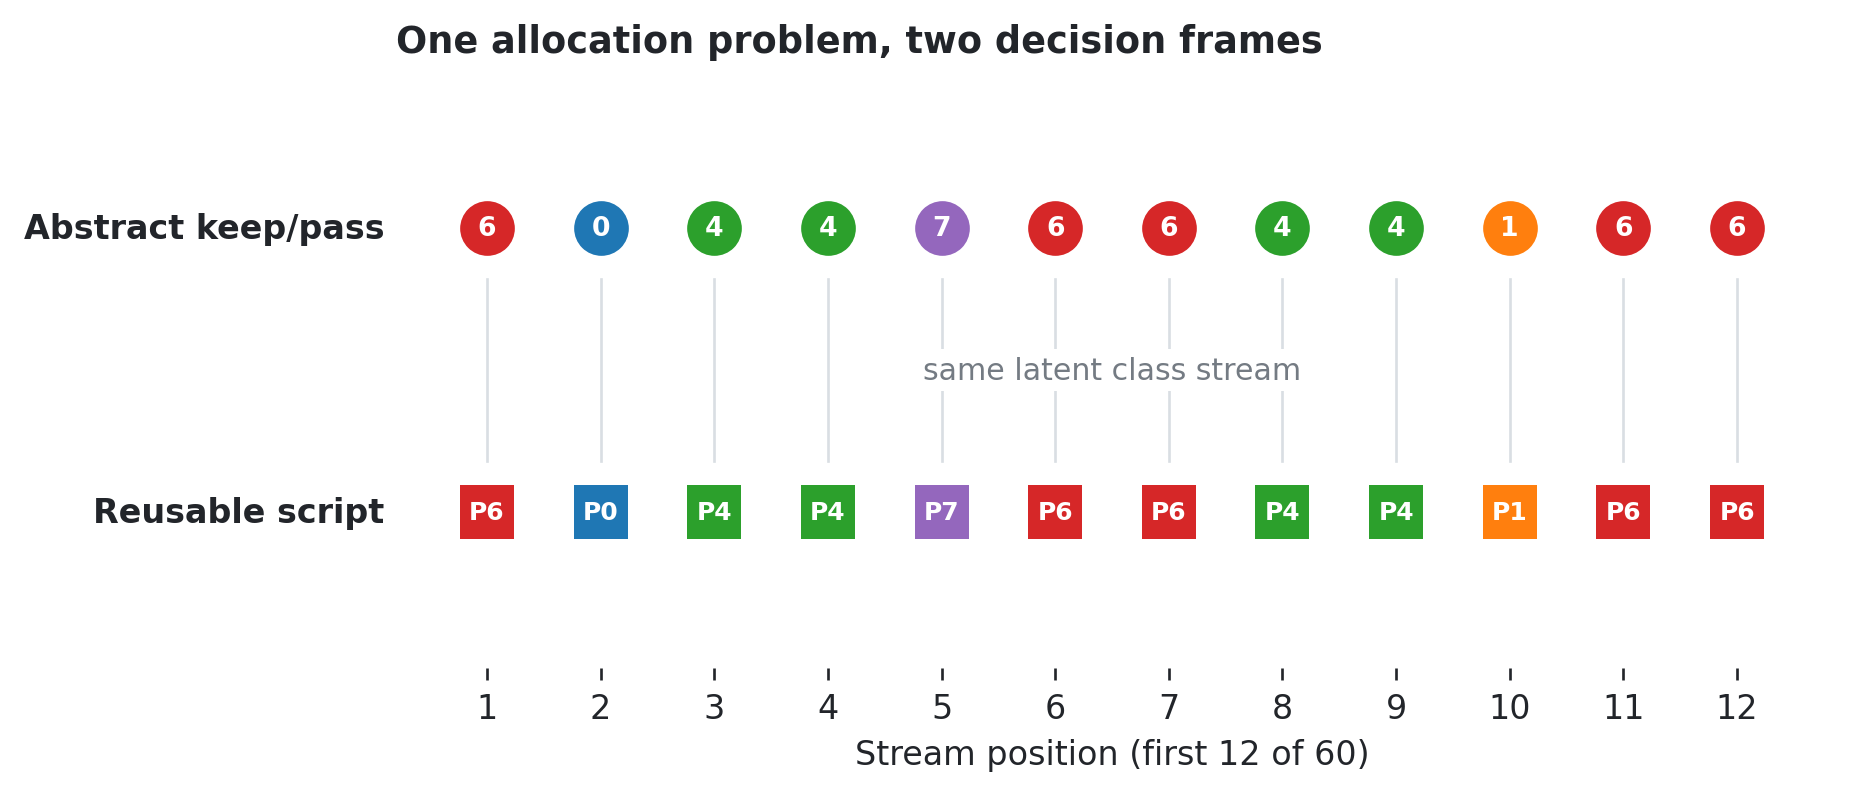
\includegraphics[width=\linewidth]{figs/fig_task_frames.png}
\caption{\textbf{One allocation problem, two decision frames.} The abstract urn
frame (top row) and the reusable-script frame (bottom row) expose the same
latent class stream; the colored circles and numeric problem families
(\texttt{P}$c$) are alternative surface representations of one shared sequence
of class identities. Colors and problem families with the same identity recur
at the same stream positions in both frames. The first 12 of 60 stream
positions are shown.}
\label{fig:frames}
\end{figure}

\textbf{The benchmark's headline comparison pairs R0 (the abstract frame
above) with R3 (the full reusable-script frame)}: the same latent allocation
problem at the two ends of the representational range, measured by behavioral
timing, which is well-defined whether or not the constructed scripts work.
Between these endpoints, a preregistered framing ladder
(Section~\ref{sec:ladder}) supplies intermediate rungs -- a declarative solver
claim on the real problem content (R1) and required-but-ungraded code emission
(R2) -- that localize which representational feature drives any observed
shift. R2 plays a second role: because it shares R0's action space, budget,
and realized payoff and never executes or rewards the emitted code, the
R0/R2 pair isolates the allocation decision from coding skill, and it is the
pair on which we report the scored outcome (Score, below). R3 additionally
depends on script correctness, so its primary outcome is timing rather than
Score.

Every condition tells both the model and the reference that exactly $N=8$
classes occur (the A2 condition). This disclosure is required for the
comparison to be same-information: the Bayesian reference's
Dirichlet-multinomial predictive is constructed with exact $N$, so a model
not told $N$ would face a strictly harder inference problem than the
reference it is scored against.

\subsection{Outcomes and references}
\label{sec:outcomes}

Our primary outcomes are behavioral timing measures:
\begin{itemize}
    \item \textbf{First-sight commitment}: the proportion of realized
    commitments made on a class's first occurrence.
    \item \textbf{First-sight hazard}: commitments on eligible first-occurrence
    turns divided by eligible first-occurrence turns.
    \item \textbf{Lateness}: the occurrence index at commitment minus the
    class's first occurrence; zero denotes immediate commitment.
\end{itemize}

For the original urn experiment, we use an exact finite-horizon Bayesian policy
with a symmetric Dirichlet prior as a labeled behavioral comparator. It is
Bayes-optimal for that prior, not for the engineered generator. For economic
regret we instead use an exact hindsight net optimum. On a realized stream, a
class of size $s_c$ built at first sight contributes $s_c-K$; the hindsight
reference chooses up to $B$ classes with the largest positive values. This
reference is prior-free and provides an offline upper bound, not an online
policy available to the model.

\paragraph{Score.} First-sight commitment and lateness are process measures:
they describe when a model commits, not whether committing paid off. We
additionally report \textbf{Score}, a single comprehensive, bigger-is-better
outcome: the competitive ratio of a policy's realized net utility to the exact
hindsight-optimal net utility on the same realized stream, pooled across seeds,
\[
\text{Score} = \frac{\sum_i \text{collected}_i}{\sum_i \text{optimal}_i}
\times 100\%,
\]
where $\text{collected}_i$ is the policy's realized net utility on seed $i$ and
$\text{optimal}_i$ is the hindsight optimum defined above, both at the
benchmark's core $B=3,K=0$ setting. Score is bounded above by 100\% by
construction (no online policy can beat the hindsight optimum) and folds both
timing (lateness cost) and allocation-target accuracy (whether the committed
classes are actually the highest-value ones) into one number, which first-sight
commitment cannot distinguish: two policies with identical first-sight rates
can have very different Scores if one of them commits to the wrong classes.
We report Score only for the R0/R2 pair (Section~\ref{sec:ladder} defines
R2): both share R0's action space and payoff structure and
neither depends on executing or grading code, so Score isolates allocation
skill from coding skill. R3 additionally requires a working script to realize
its credited value, which would conflate the two, so the headline R0/R3
dissociation is measured by timing and Score supplements it on the R0/R2
pair.

\subsection{Experimental protocol}

The primary controlled subject is Claude Haiku 4.5. Claude Opus 4.8 provides a
frontier-model paired test plus an R2 code-emission bridge. Qwen2.5-Coder-14B
is used for reward learning.
GPT-5.4-mini and GPT-5.6 Sol are evaluated under a preregistered competence gate
with matched R0 and R2 conditions and \texttt{reasoning\_effort=none}.

Core Haiku, Opus, and GPT comparisons use 24 canonical streams (seeds
2000--2023): the original 12 preregistered streams (2000--2011) plus a
seed-extension panel (2012--2023) added post hoc to tighten the bootstrap
intervals, run under the identical generator, prompts, and harness.
Repeated conditions on these streams are not independent samples: the effective
stream sample is 24, not the number of sessions. The final Qwen transfer test
uses 24 paired held-out streams (2000--2023), disjoint from training seeds.
The Opus script arm uses the same 24 canonical latent streams and the same
magnitude-100 numeric rendering as Haiku and both GPT models, so all four
models answer literally identical problem instances under R3, closing the one
remaining asymmetry in the model panel. A preflight structural projection
assertion passes on all 24 seeds. Josephus remains partly hand-solvable for
Opus at any magnitude; we therefore treat Opus timing as the primary paired
outcome, report a Josephus-excluded sensitivity, and do not use its script-arm
regret as a payoff-isomorphic cross-frame estimate.
Appendix~\ref{app:magnitude-sensitivity} additionally reports Opus's R3 arm
under the magnitude-1000 pool used earlier in this project to foreclose
Opus's partial hand-solving ability, retained for completeness: the timing
result is unchanged within the seed-bootstrap interval.
We report numerators and denominators, pooled arm summaries, and mean paired
seed differences. Unless stated otherwise, 95\% intervals resample paired
seeds with replacement 10,000 times and take the 2.5th and 97.5th percentiles
of the bootstrap distribution. For first sight among realized commitments, a
seed with zero commitments has an undefined proportion and is excluded from
that estimand; first-sight hazard, commitment count, and zero-commit incidence
remain defined and are reported alongside it. Economic interactions are
computed within seed before resampling.

Mechanical validity is checked independently of behavioral outcomes. The
harness asserts stream hashes, separates transport failures from model
decisions, records malformed and unknown tool calls, and checks token-cap
truncation. Only mechanical failures permit reruns. Prompt, tool-choice, and
token-cap repairs discovered during benchmark development are documented in
the artifact record.

\subsection{Preregistered framing ladder}
\label{sec:ladder}

To localize which representational feature drives any cross-frame shift
between the R0 and R3 endpoints, we vary the decision representation in four
paired rungs:
\begin{description}
    \item[R0:] abstract free-text \textsc{keep}/\textsc{pass};
    \item[R1:] real numeric problem content with a declarative solver claim,
    through tool calls, but no code;
    \item[R2:] R1's binary claim/skip loop, budget, streams, realized payoff,
    and lack of a hand-solving option, with one protocol addition: a required
    non-empty \texttt{solve(inputs)} implementation. Payoff is deliberately
    independent of code correctness, so correctness-dependent reward cannot
    explain a timing shift at this rung;
    \item[R3:] full reusable-script construction, with scripts persisted and
    rerunnable on later instances.
\end{description}
The preregistered localization criterion is the earliest adjacent increase of
at least 30 percentage points in first-sight commitment. The ladder is coarse,
not a complete factorial design: the R0-to-R1 step bundles the shift to a
tool-call claim action with the introduction of real numeric problem content,
and the decisive R1-to-R2 contrast holds that content fixed while adding only
the required-code constraint. Ladder results appear in
Section~\ref{sec:ladder-results}.

\section{Experimental Results}
\label{sec:results}

We organize our results in logical order. In Section~\ref{sec:gate}, we establish that 
frontier models naturally possess allocation ability in the abstract frame R0, but no model preserves this ability in the 
constructive environment R3. We isolate the failure mode for most models at code 
emission (R2) in Section~\ref{sec:ladder-results}. Next, Section~\ref{sec:score-results}
presents a simple numerical metric of online allocation ability unconfounded by varying tool 
creation ability. We also include further experiments to preempt two natural questions. 
In Section~\ref{sec:economic}, we test whether models allocate differently under different
presented building costs. We find some variation under R0 but almost no response under R2. 
Finally, Section~\ref{sec:qwen-case-study} shows that the gap between R0 and R2 holds 
even in models that have been post-trained specifically to suceed at R0.

\subsection{Abstract competence but tool-budgeting failure}
\label{sec:gate}

We first show that frontier models have the ability to 
allocate budget semi-optimally in an abstract setting. We test Haiku, Opus, 
GPT-5.4-mini, and GPT-5.6 Sol on the R0 framing (see Section \ref{sec:ladder}). We find that all four frontier models reserve their 
budgets: as shown in Figure \ref{fig:core}, each waits for evidence of recurrence before committing more than $70\%$ of the time. However, this competence fails to generalize to tool allocation. Though the
R0 and R3 environments provide the models with the same information and task them with the same 24 class streams, no model waits for recurrence more than $12\%$ of the time in the latter. This shows that R3 significantly suppresses a demonstrated allocation ability in all tested models.

\begin{figure}
\centering
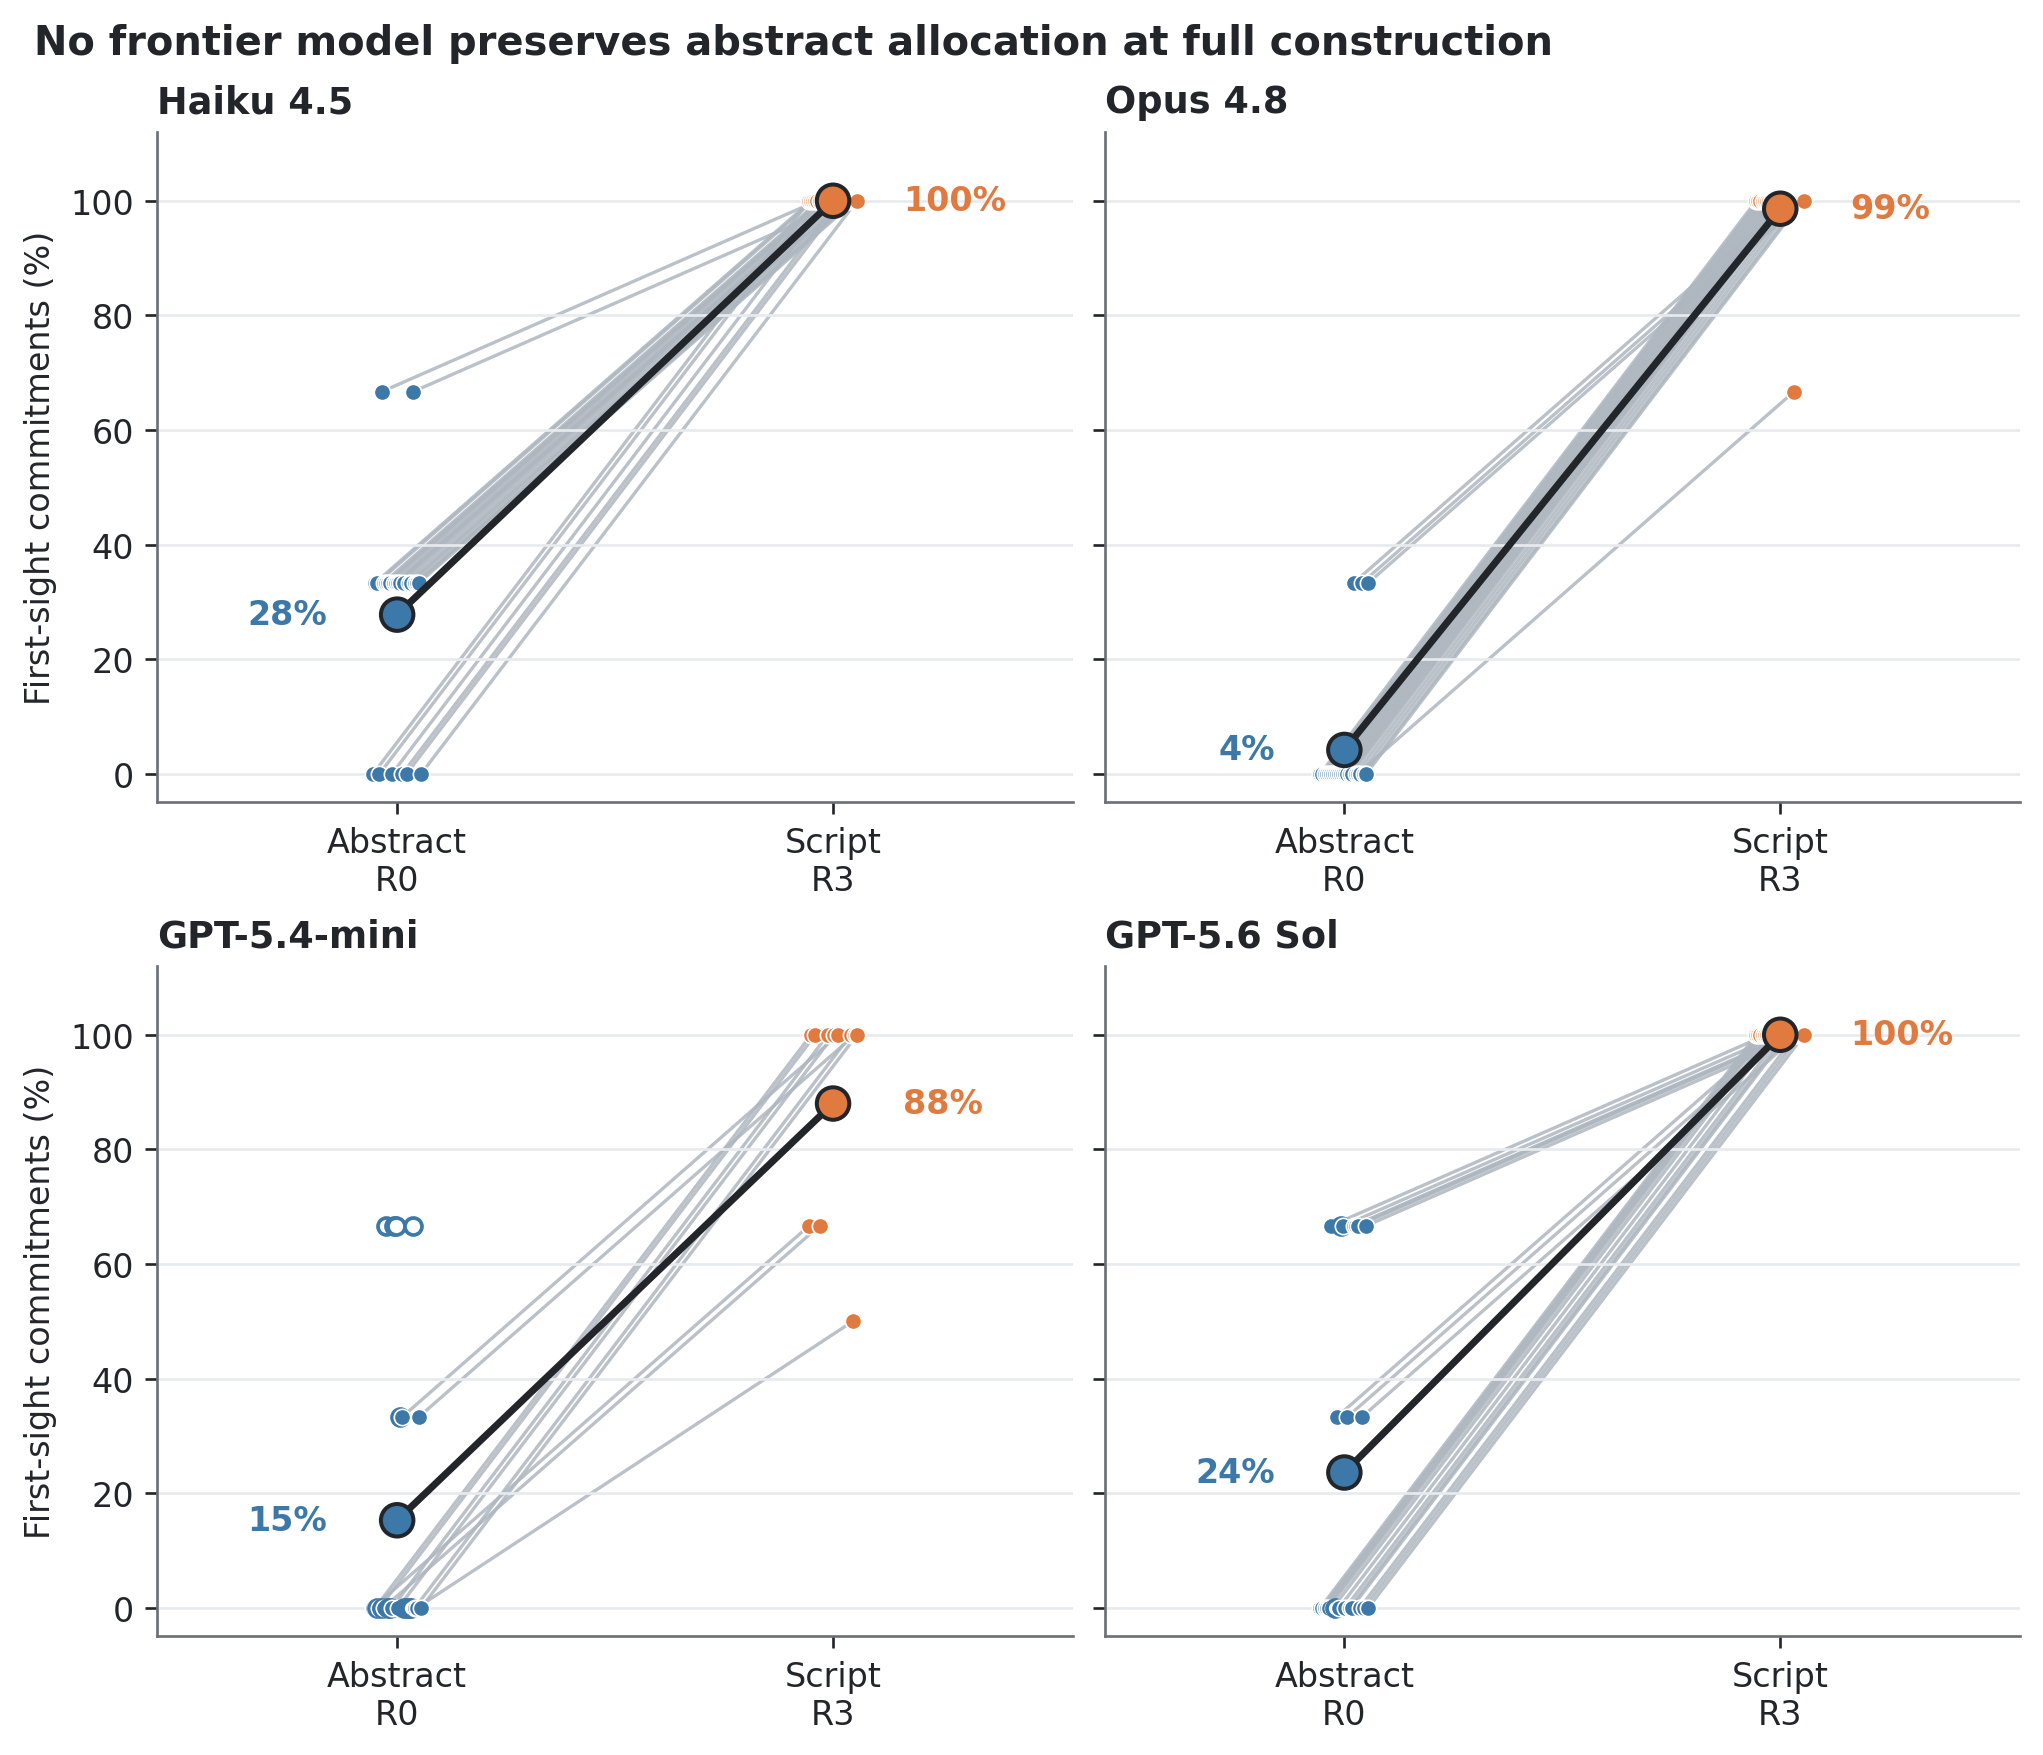
\includegraphics[width=\linewidth]{figs/fig_core_dissociation.png}
\caption{\textbf{First-sight commitment rate of frontier models on R0 and R3.} Thin lines connect paired seeds; large points show averages. Open circles mark seeds that commit in the
abstract frame but realize no script build at all in R3.}
\label{fig:core}
\end{figure}

The models' reasoning transcripts in the two frames help to explain the differences in their behavior. Abstract decisions prompt
references to recurrence and budget preservation: in one stream, Opus says, \textit{Still gathering information;
too early to commit a keep.} This is mirrored by the other models and reflects the intended behavior of committing only once a type's rate is
established (\textit{Red has now appeared 3 times in 7 draws --- a strong rate.
With 53 draws left, keeping red should yield many more.}) In contrast, the tool frame causes models to fixate on the immediate instance. For example, Opus states on the first problem of a stream, \textit{I'll write a script for this bit-manipulation
problem type.} Budget is only mentioned near exhaustion (\textit{I have 1 write left. Let me use it for this LCG
type which may recur.}) The models do not consider waiting for recurrence evidence at all, and scripts are reused only reactively when a class later returns. For fuller per-seed excerpts, see Appendix~\ref{app:transcripts}.

\begin{comment}
In contrast, Qwen2.5-Coder-14B displays first-sight commitment almost 3 times
higher than all the frontier models. This shows that our later results represent the suppression of a demonstrated capability, not the complete absence of one. 

\begin{table}[H]
  \centering
  \label{tab:first-sight}
  \begin{tabular}{|l|r|}
  \hline
  Model & First-sight commitment\\
  \hline
  Haiku & 28\% \\
  Opus & 4\% \\
  GPT-5.4-mini & 15.3\% \\
  GPT-5.6 Sol & 23.6\% \\
  \textbf{Qwen2.5-Coder-14B} & \textbf{74\%} \\
  \hline
  \end{tabular}
\caption{First-sight commitment of frontier models and base Qwen on abstract framing R0.}
\end{table}

Haiku has a first-sight commitment of 28\% of realized commitments (20/72, mean lateness
1.39), Opus on 4\% (3/72), GPT-5.4-mini on 15.3\% (first-sight hazard 8.0\%),
and GPT-5.6 Sol on 23.6\% (mean lateness 1.08, collecting 99.8\% of the
Bayesian comparator's payoff). Each waits for recurrence evidence before
spending budget and realizes 75--86\% of the hindsight-optimal net utility
(Table~\ref{tab:score}). Untrained Qwen2.5-Coder-14B fails this gate -- it is
eager in the abstract frame as well (74\% first sight) -- which motivates the
reward-learning case study of Section~\ref{sec:qwen-case-study}; its
RL-trained policy (35\% first sight) passes. Every eager constructive result
below is therefore the suppression of a demonstrated policy, not the absence
of one.

Haiku receives the same class-count information and acts on the same class
streams in both frames, yet waits in the abstract task (28\% first sight,
lateness 1.39, regret $74\pm216$ against the Bayesian comparator) and commits
immediately when the action is reusable script construction (100\% first
sight, lateness 0.00, regret $1477\pm395$). The same pattern -- an abstract
reserve policy that does not survive R3 -- appears in every model and family
we test, including the reward-trained Qwen policy
(Section~\ref{sec:qwen-case-study}). Table~\ref{tab:models} and
Figure~\ref{fig:capability-map} summarize the panel. We state the shared
result at the level the data support: \textbf{no tested model preserves its
abstract allocation policy under full reusable-script construction}. The way
the policy fails, however, differs sharply by model, and the differences are
themselves informative.

\begin{table}[t]
\centering
\caption{The R0/R3 dissociation across the competence-gated panel. Entries are
pooled first-sight proportions among realized commitments; R3 is full
reusable-script construction. Haiku, Opus, and the
GPT models are reported at $N=24$ (seeds 2000--2023). Both GPT R3 entries are
conditional on commitment. GPT-5.4-mini realizes only 25/72 (34.7\%) of
available write-budget slots across the panel, with 13/24 seeds (54.2\%)
realizing zero commitments; realized commitments are nonetheless as eager as
Haiku's and Opus's (88.0\% first sight). GPT-5.6 Sol realizes 53/72 (73.6\%)
of slots, with 2/24 zero-commit seeds; its realized commitments are eager to
ceiling (100\% first sight) and cluster entirely within each session's first
11 problems, with no later or reconsidered builds. All R0/R3 cells for
every model use the
identical magnitude-100 numeric rendering, so every model answers literally the
same problem instances; Appendix~\ref{app:magnitude-sensitivity} reports a
magnitude-1000 completeness check for Opus's R3 arm. Per-model R2 localization
and R3 failure mode are summarized in Table~\ref{tab:ladder}
(Section~\ref{sec:ladder-results}).}
\label{tab:models}
\small
\begin{tabular}{@{}lrr@{}}
\hline
Model & R0 & R3 \\
\hline
Haiku 4.5 & 28\% & 100\% \\
Opus 4.8 & 4\% & 98.6\% \\
GPT-5.4-mini & 15.3\% & 88.0\% \\
GPT-5.6 Sol & 23.6\% & 100\% \\
\hline
\end{tabular}
\end{table}

\begin{figure}[t]
\centering
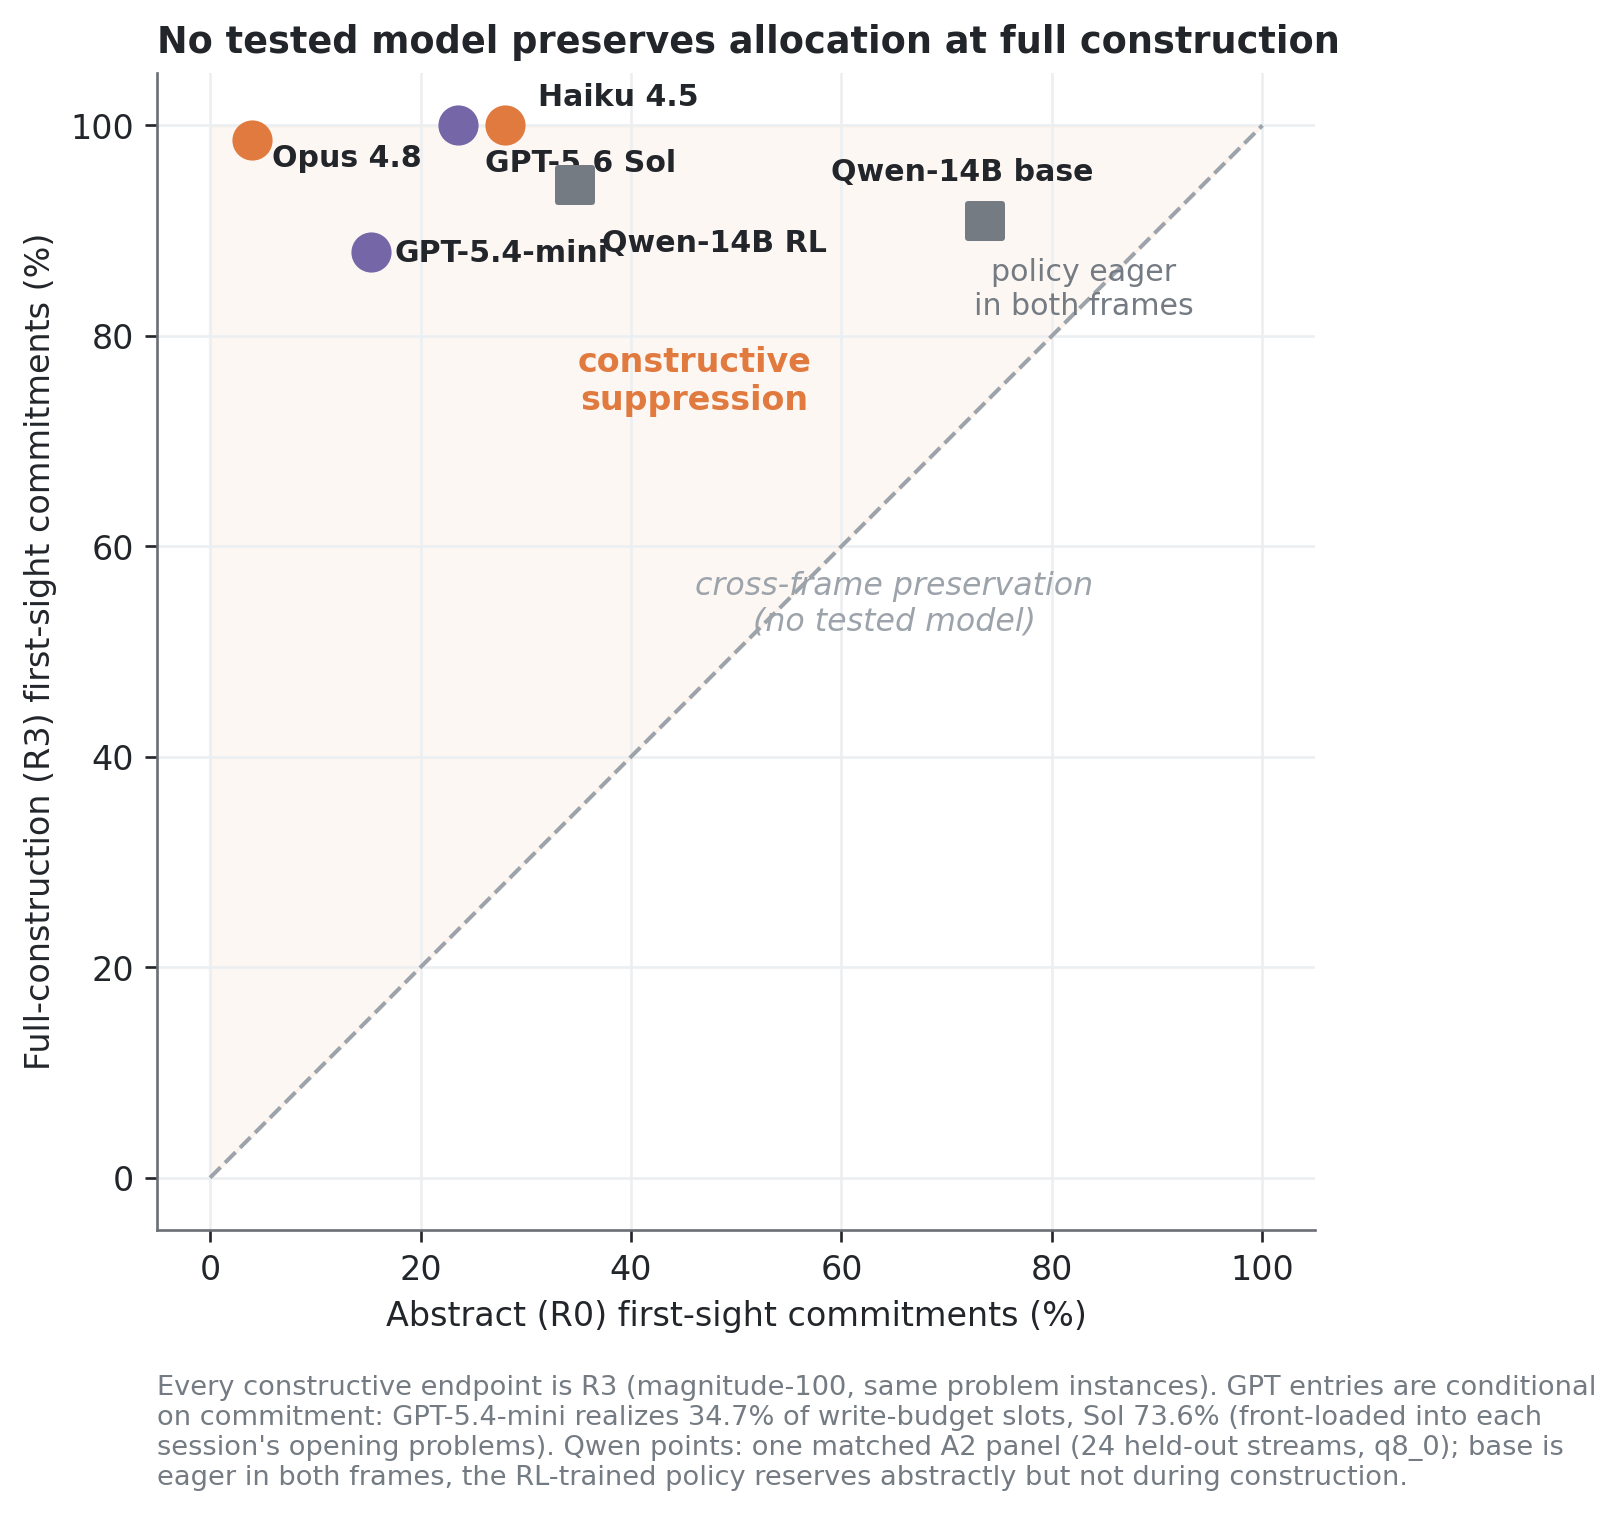
\includegraphics[width=0.78\linewidth]{figs/fig4_capability_map.png}
\caption{\textbf{No tested model preserves abstract allocation at full
construction.} The diagonal denotes preservation of first-sight timing across
the abstract and full-construction frames; every plotted constructive
endpoint is R3, rendered at the same magnitude-100 numeric pool so every
model faces the same problem instances. All models lie far above the
diagonal. GPT entries are conditional on commitment and understate the
divergence in realization: GPT-5.4-mini realizes only 34.7\% of its available
write-budget slots and GPT-5.6 Sol 73.6\% (Table~\ref{tab:models}); Sol's
ceiling-eager builds are additionally front-loaded into each session's
opening problems. Both Qwen-14B points come from one matched A2 evaluation
panel (24 held-out streams, q8\_0): the untrained base is eager in both
frames (policy absence), while the RL-trained policy reserves abstractly but
not during construction (acquisition without activation).}
\label{fig:capability-map}
\end{figure}

Opus's collapse is the cleanest. It reserves almost completely in the urn
(4\% first sight, 3/72 commitments), yet under full R3, rendered at magnitude
100 -- the
identical problem instances answered by Haiku, GPT-5.4-mini, and GPT-5.6 Sol,
rather than the magnitude-1000 pool used earlier in this project specifically to
foreclose Opus's partial hand-solving ability -- 71 of 72 script builds occur at
first sight (98.6\%), mean lateness 0.014; the single non-first-sight build
(modpow, seed 2018) commits at class position 2. The R3-minus-R0 paired
difference is $+94.4$ points, with a 95\% seed-bootstrap interval
$[+88.9,+98.6]$ -- no longer degenerate at $N=24$, since Opus R0 no longer
reserves on literally every seed, but still reflecting a near-total framing
shift. Josephus accounts for seven of the 72 R3 builds, all of them at first
sight; excluding it leaves 64/65 first-sight builds (98.5\%), so the one
non-first-sight build is unrelated to Josephus's known hand-solvability. Across
the full 24-seed panel, Opus submitted a raw, script-free answer to an unbuilt
class only once, and that attempt was incorrect, despite facing the same
magnitude at which its own calibration shows roughly 25--38\% hand-solve
accuracy in isolation. Thus the R3 result is not an artifact of the
magnitude-1000 hardening used elsewhere: at matched magnitude, with a genuine
if narrow hand-solve alternative on the table, Opus's construction-time
eagerness is essentially unchanged (Appendix~\ref{app:magnitude-sensitivity}).
Haiku's R3 arm behaves identically (100\% first sight, lateness 0.00).

GPT-5.4-mini loses the policy by the opposite route. Only 25 of
the 72 possible write-budget slots are ever exercised (commits per seed 1.04),
and 13/24 seeds (54.2\%) realize zero script builds despite each stream
presenting up to eight recurring problem types. Conditional on committing at
all, however, GPT-5.4-mini is
eager: 22/25 realized commitments (88.0\%) occur at first sight, with pooled
lateness 0.12 among realized builds, comparable to Opus's 0.083. The
unconditional first-sight hazard is 12.3\% (22/179); this denominator is
large because non-committing R3 sessions run the entire
60-problem stream rather than truncating at budget exhaustion, so they expose
many more eligible first-occurrence turns. Neither behavior preserves the
abstract policy: a recurrence-conditioned reserve policy predicts \emph{late}
commitment, which GPT-5.4-mini exhibits on no seed. The degenerate pattern is
consistent with a reasoning-policy explanation specific to this snapshot:
OpenAI's Chat Completions endpoint rejects function-tool calls at
\texttt{reasoning\_effort=low} for \texttt{gpt-5.4-mini-2026-03-17}, forcing
\texttt{reasoning\_effort=none} in both arms. Absent visible deliberation,
whichever action -- \texttt{write\_script} or the always-available
\texttt{submit\_answer} -- is emitted on a session's first problem or two
appears to persist for the remainder of the stream, with no observed
within-session revision even after dozens of exposures to a recurring type
and near-zero measured accuracy. All 24 R3 sessions are mechanically clean
(zero malformed, unknown, or refused tool calls).

GPT-5.6 Sol fails latest and most revealingly. It realizes 53 of the 72
possible write-budget slots
(73.6\%), with 2/24 seeds (8.3\%) realizing zero commitments -- a much smaller
shortfall than GPT-5.4-mini's. But every
realized commitment (53/53, 100\%) occurs at first sight with zero lateness,
and the eagerness is not simply
increased confidence: by raw stream position rather than class-relative
position, all 22 of Sol's committing seeds write their first script on the
session's very first problem, and every realized build across the panel falls
within the first 11 problems of the 60-problem stream, with no later writes
and no observed reconsideration. Haiku and Opus show the identical early-slot
clustering on these same canonical streams -- the generator guarantees early
exposure to the recurring types, so clustering itself is expected, not
anomalous. What is specific to Sol is the absence of any \emph{later}
commitment, in sharp contrast to its genuinely spread, sometimes-delayed R2
claims (Section~\ref{sec:ladder-results}). Sol's R3 behavior is a
front-loaded,
non-revisited batch of construction decisions made in the session's opening
turns. All 24 R3 sessions are mechanically clean
(zero malformed, unknown, or refused tool calls); 12/24 truncate on budget
exhaustion and 12/24 on the 300,000-token session cap.

Three failure modes, one shared outcome. Whether by eager per-class collapse
(Haiku, Opus), degenerate under-commitment with eager realized builds
(GPT-5.4-mini), or a front-loaded, never-revisited opening batch (Sol), the
recurrence-conditioned defer-then-confirm policy that every model demonstrates
in R0 is not expressed at R3 -- and Section~\ref{sec:qwen-case-study} shows
the same holds for a policy installed directly by reward. The claim is scoped
to the models and families tested, and these comparisons do not identify what
causes the differences in failure mode: post-training, architecture,
reasoning policy, and tool-use
experience all remain possible explanations.
\end{comment}


\subsection{Localizing the trigger: the framing ladder}
\label{sec:ladder-results}

Which representational rung triggers the collapse? We run the full ladder
(Section~\ref{sec:ladder}) on all four frontier models across the same 24
paired A2 streams (seeds 2000--2023). Table~\ref{tab:ladder} reports pooled
first-sight commitment among realized commitments at each rung.

\begin{table}[t]
\centering
\caption{Framing ladder across the frontier panel: pooled first-sight
commitment (\%) among realized commitments at each rung (24 paired A2
streams, seeds 2000--2023), with each model's R3 failure mode. R0 is abstract
\textsc{keep}/\textsc{pass}; R1 a declarative solver claim on the real problem,
no code; R2 the same claim/skip loop with a required non-empty
\texttt{solve(inputs)} implementation whose payoff is independent of code
correctness; R3 full reusable-script construction. GPT-5.4-mini's R1 rate is
among its few realized claims (0.71 claims/seed; 17/24 seeds claim nothing),
and both GPT R3 entries are conditional on commitment (GPT-5.4-mini realizes
only 34.7\% of available build slots). The eagerness trigger sits at required
code emission (R2) for Haiku, Opus, and (in its degenerate form)
GPT-5.4-mini, and only at full construction for GPT-5.6 Sol.}
\label{tab:ladder}
\small
\begin{tabular}{@{}lrrrrp{3.6cm}@{}}
\hline
Model & R0 & R1 & R2 & R3 & R3 failure mode \\
\hline
Haiku 4.5    & 28   & 33 & 100  & 100  & Eager collapse (trigger: R2) \\
Opus 4.8     & 4    & 0  & 91.7 & 98.6 & Eager collapse (trigger: R2) \\
GPT-5.4-mini & 15.3 & 29 & 85.0 & 88.0 & Degenerate under-commitment; eager when committing \\
GPT-5.6 Sol  & 23.6 & 0  & 38.9 & 100  & Front-loaded batch (trigger: full construction) \\
\hline
\end{tabular}
\end{table}

The pattern is shared across the panel and isolates the same trigger. In the
abstract frame (R0) every model reserves, committing at first sight only
4--28\% of the time. A declarative solver claim on the real numeric problem
(R1) --- a tool-call action carrying a current-plus-future commitment, but no
code --- does not reproduce eagerness in any model: Haiku rises only to 33\%,
Opus and Sol stay at 0\%, and GPT-5.4-mini both under-commits severely (0.71
claims per seed, 17 of 24 seeds claiming nothing) and is only moderately eager
on the claims it does make (29\%). The jump arrives at R2, whose sole added
ingredient is a required non-empty \texttt{solve(inputs)} implementation with
payoff still independent of code correctness: first-sight commitment leaps to
100\% (Haiku), 91.7\% (Opus), and 85.0\% (GPT-5.4-mini). Full construction
(R3) then holds every model at or near ceiling (88.0--100\%). GPT-5.6 Sol is
the panel's exception and its construct-validity control: it withstands the
required-code rung (38.9\% at R2, claims genuinely spread across turns) and
collapses only at full construction (100\% at R3), showing that code emission
does not \emph{mechanically} force eagerness and that the code-required
allocation task is itself passable.

Haiku, the primary controlled subject, makes the localization sharpest. Its
mean claim lateness falls from 1.389 (R0) and 0.847 (R1) to 0.000 at both R2
and R3, and the paired adjacent first-sight differences (95\% seed-bootstrap
intervals, $N=24$) place the entire jump at the required-code rung: R1--R0
$=+5$ points (descriptive), R2--R1 $=+66.7$ $[+51.4,+80.6]$, and R3--R2 $=0.0$
$[0.0,0.0]$. Full construction adds nothing beyond required code emission; the
final degenerate interval reflects ceiling observations in both rungs, not a
general equivalence claim. These descriptive intervals do not replace the
preregistered 30-point localization rule and are not multiplicity-adjusted.
Figure~\ref{fig:ladder} displays the paired stream trajectories.

\begin{figure}[t]
\centering
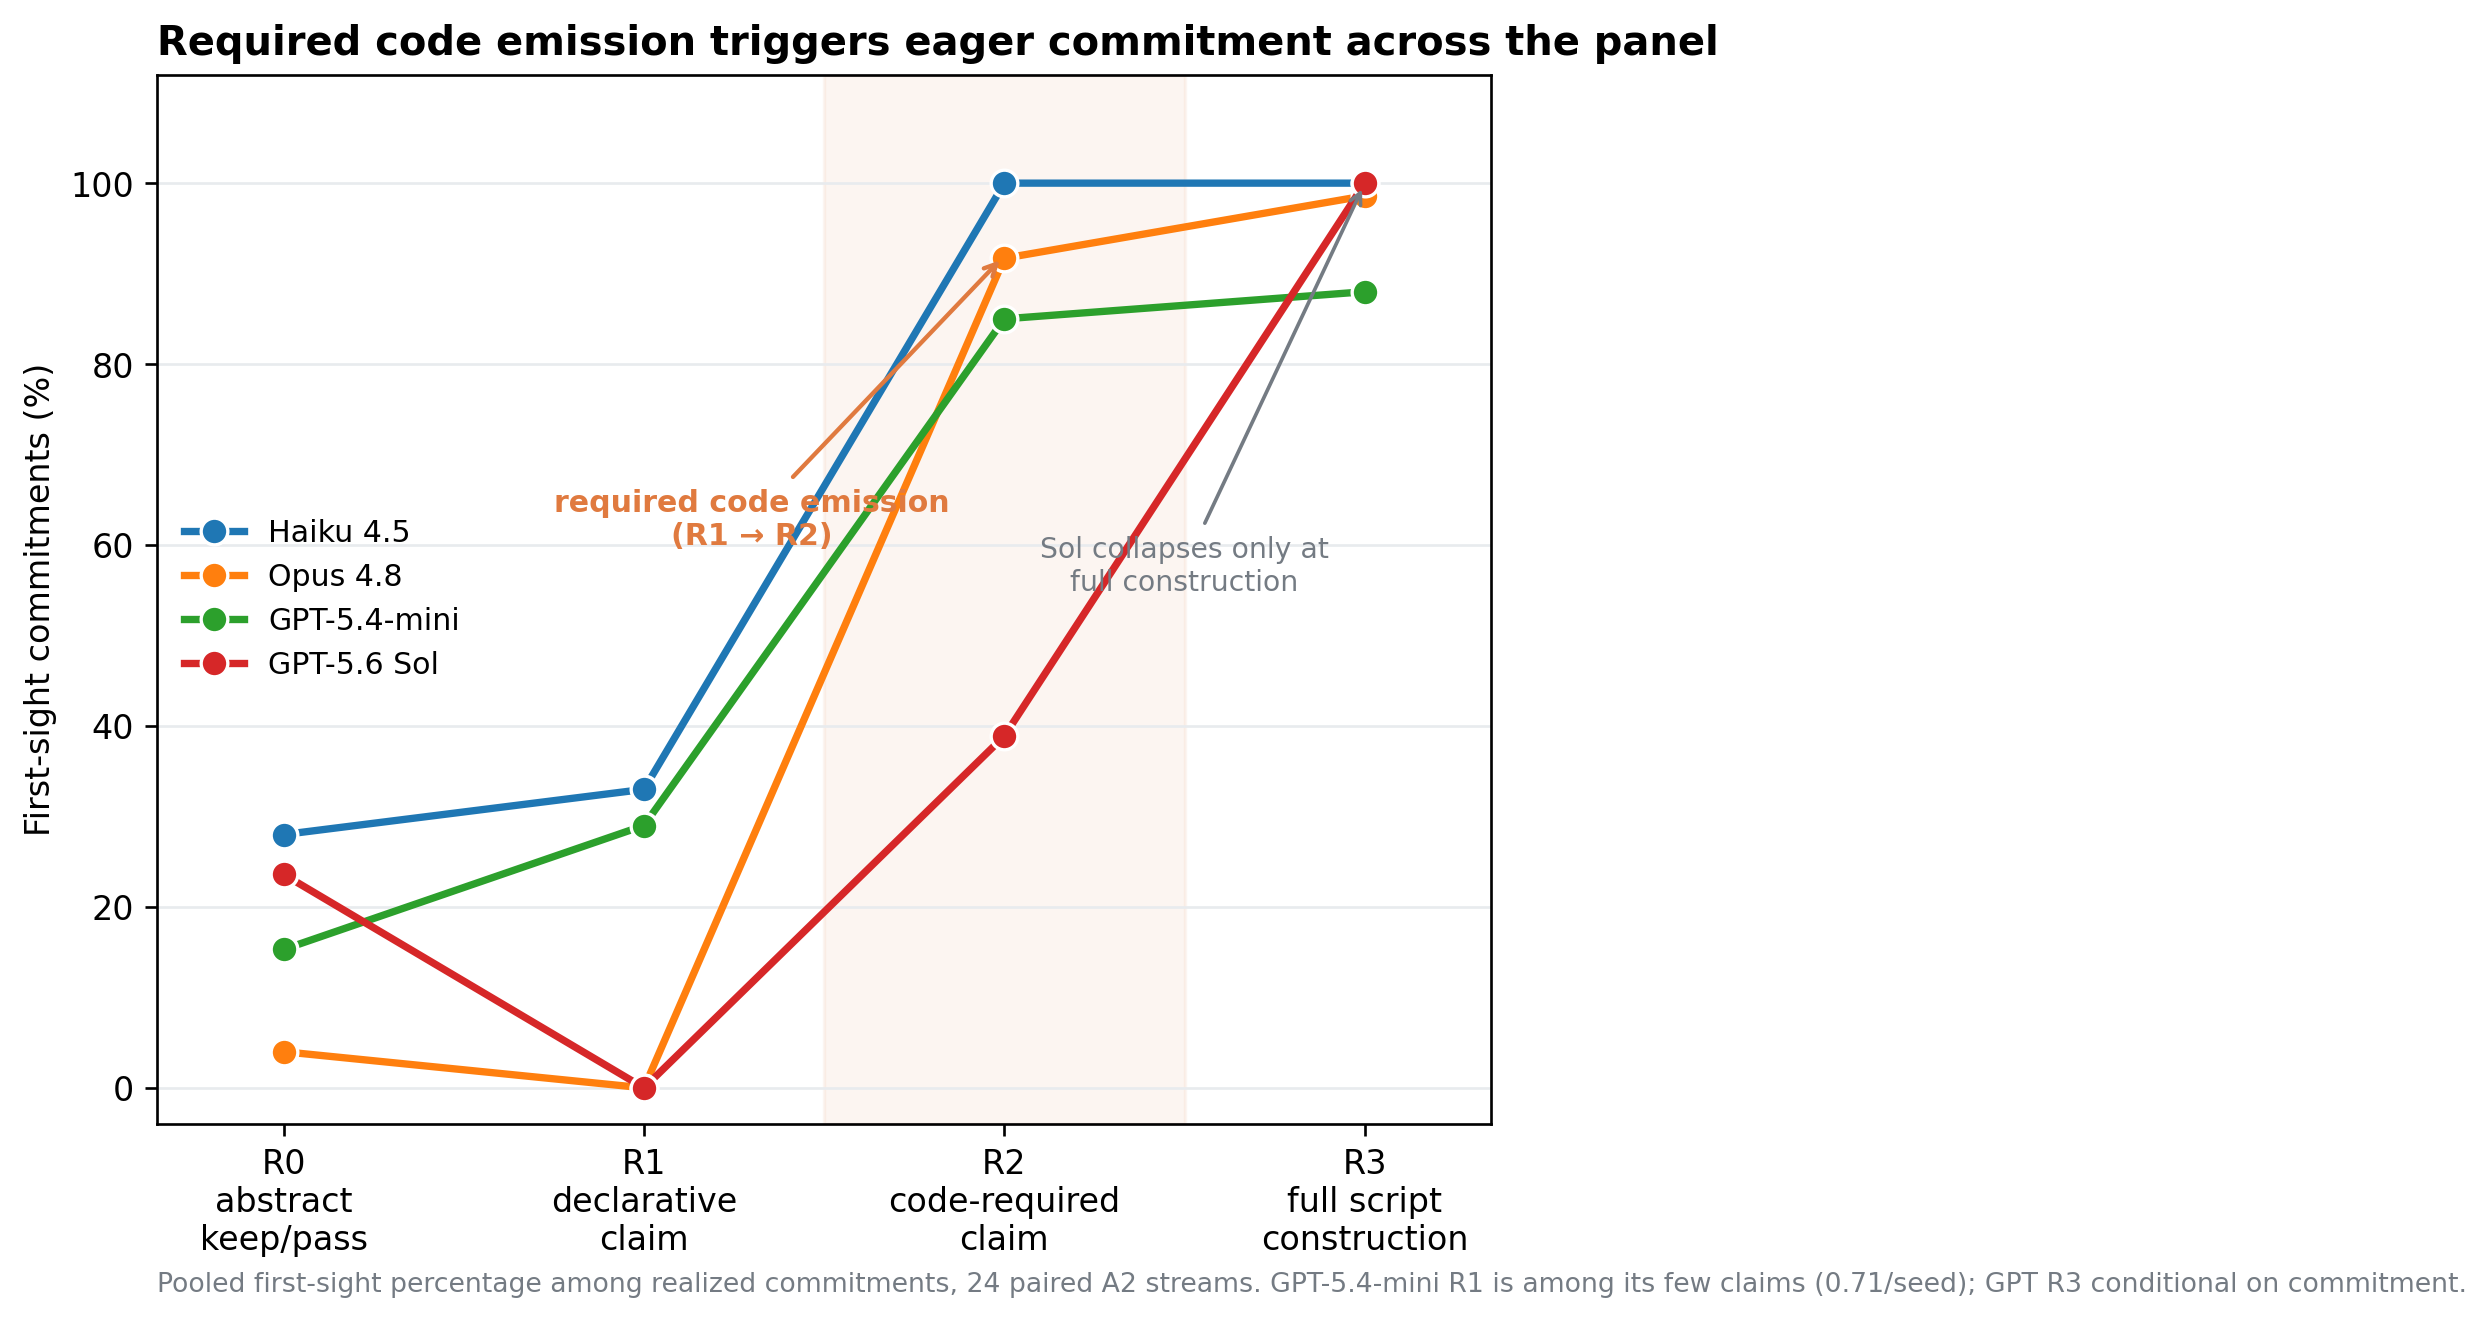
\includegraphics[width=\linewidth]{figs/fig2_framing_ladder.png}
\caption{\textbf{Preregistered framing ladder and construction-only control.}
Thin lines connect the same 24 canonical streams across conditions; large
points show pooled first-sight commitment. A declarative solver claim on the
real problem (R1) does not reproduce full eagerness. Requiring code
while preserving R1's realized payoff and removing correctness-dependent reward
(R2) raises
first-sight commitment to ceiling for Haiku, Opus, and GPT-5.4-mini, matching
full script construction (R3).}
\label{fig:ladder}
\end{figure}

Within this benchmark, required code emission is therefore sufficient to
reproduce the full effect for Haiku, Opus, and GPT-5.4-mini; the declarative
claim, correctness-dependent reward, and a hand-solving escape valve are not
necessary. The design does not distinguish emission itself from the compliance
or effort induced by an instruction to produce correct code.
Code quality provides a secondary diagnostic. Only 12 of 789 tested R2
instances (2\%) are correct, and 61 of 72 claimed solvers are degenerate across
their class. Inspection shows structurally plausible code that hard-codes
incidental parameters from the current instance instead of using the input
fields. This suggests current-instance fixation, but correctness is post hoc
and does not enter the causal R1/R2 comparison.

The R2 trigger replicates in Opus, which becomes nearly eager as soon as
code emission is required: it makes all 72 available claims, 66 at first
sight (91.7\% among commitments; first-sight hazard 66/77 = 85.7\%), with
mean lateness 0.083; its mean net score is 32.7 and regret against the exact
hindsight net optimum is $17.0\pm1.2$. Together with its R3 arm, this
localizes Opus's shift to required code emission, replicating Haiku's ladder
boundary. GPT-5.4-mini rises from
15.3\% R0 to 85.0\% R2 first-sight commitment; the paired difference is
$+73.3$ points with a 95\% bootstrap interval of $[+58.3,+86.7]$. Seed-level
heterogeneity remains: one R2 seed (2007) waits substantially (mean lateness
4.33) and four make no commitments. The displayed arm rates are pooled ratios:
$11/72-51/60\approx69.7$
points. The $+73.3$-point inferential estimand instead averages the 20
within-seed differences for which both among-commitment proportions are
defined; the four zero-commit R2 seeds are excluded from that conditional
estimand. R0 and R2 hazards are 8.0\% and 47.2\%, respectively; this
unconditional analysis retains the zero-commit seeds. Its degenerate R3
under-commitment (Section~\ref{sec:gate}) localizes one rung further:
paired against R2 on the same
seeds (10,000-resample seed-bootstrap, RNG seed 0, matching
Section~\ref{app:bootstrap}), zero-commit incidence rises by $+37.5$ points
$[+12.5,+62.5]$ and commits per seed fall by $-1.46$ $[-2.13,-0.75]$, while
first-sight timing conditional on commitment is statistically indistinguishable
between the two arms ($+5.6$ points $[-16.7,+33.3]$, $n=9$ seeds committing in
both): required code emission does not reliably restore
commitment itself, but conditional on emission the timing is the same
near-immediate eagerness seen in the other models.

GPT-5.6 Sol is the exception at this rung, and the exception is what
validates the instrument. Sol remains selective when code is required: R0 and
R2 first-sight rates are 23.6\% and 38.9\%, with mean
lateness 1.08 and 0.90. The paired difference is $+15.3$ points with a 95\%
interval of $[+0.0,+30.6]$ -- below the preregistered suppression criterion,
though the interval does not establish equivalence of the two arms. Sol's
R2 claims are genuinely spread across turns 0--9 and sometimes occur after a
type has already recurred once or twice; its collapse arrives only at full
construction, where the paired R2-to-R3 change is $+57.6$ points
$[+42.4,+71.2]$ (same seed-bootstrap procedure, Section~\ref{app:bootstrap}),
with commits per seed falling by $-0.79$ $[-1.21,-0.42]$ and zero-commit
incidence rising by $+8.3$ points $[+0.0,+20.8]$. Sol's R2 selectivity is
the panel's construct-validity control: required code generation does not
mechanically force eagerness, and the code-required allocation task is
passable by a current model. The universal failure of
Section~\ref{sec:gate} therefore reflects a capability boundary at
full construction, not an impossible task -- with the trigger sitting at
code emission for Haiku, Opus, and (in its degenerate form) GPT-5.4-mini,
and at full construction for Sol.

\subsection{Allocation quality: Score}
\label{sec:score-results}

First-sight commitment describes timing only: a model can commit immediately
yet to the wrong classes, or wait and still misallocate.
Table~\ref{tab:score} reports \textbf{Score} (Section~\ref{sec:outcomes}),
the pooled competitive
ratio against the exact hindsight optimum at $B=3,K=0$, so 100\% is the ceiling
and bigger is better throughout, on the scored R0/R2 pair for every model
with both arms collected.

\begin{table}[h]
\centering
\caption{Score: percent of the exact hindsight-optimal net utility realized,
pooled over 24 canonical seeds ($B=3,K=0$), on the scored R0/R2
pair. Bigger is better. Qwen's R2 cells pool every realized outcome across
all 24 seeds with no seed exclusions, including seeds on which the model's
own idle-tail generation failure (Section~\ref{sec:qwen-case-study};
Appendix~\ref{app:mech-validity}) left its write budget only partially spent;
we report the unfiltered outcome rather than a filtered subset to avoid
biasing the comparison toward whichever arm happens to fail less often.}
\label{tab:score}
\begin{tabular}{lrr}
\hline
Model & R0 score & R2 score \\
\hline
Haiku 4.5 & 77.6\% & 66.2\% \\
Opus 4.8 & \textbf{86.0}\% & 65.9\% \\
GPT-5.4-mini & 75.1\% & 54.2\% \\
GPT-5.6 Sol & 78.3\% & \textbf{78.4}\% \\
Qwen-14B base (q8) & 74.8\% & 61.2\% \\
Qwen-14B RL-final (q8) & 80.4\% & 61.2\% \\
\hline
\end{tabular}
\end{table}

Score changes which comparisons look striking. GPT-5.6 Sol's R2 score
(78.4\%) is the panel's best, consistent with
Section~\ref{sec:ladder-results}: R2 under-elicits Sol's suppression, which
appears only at R3 -- a rung on which Score is undefined because credited
value would additionally depend on script correctness. A high R2 Score is
therefore evidence about the rung, not about cross-frame preservation.
Decomposing Score into budget utilization and
allocation-target accuracy shows GPT-5.4-mini's R2 shortfall (54.2\%) is
driven roughly equally by leaving optimal build slots unclaimed and by
misallocating the slots it does spend, not primarily by timing. Opus and
Haiku's R2 scores (65.9\% and 66.2\%) sit well below their own R0 scores (86.0\%
and 77.6\%) despite reaching or approaching ceiling first-sight commitment in
R2: acting immediately is not the same as acting on the right classes. The
RL-trained Qwen-14B policy's R0 score (80.4\%, versus 74.8\% for its untouched
base) is a substantially cleaner statement of the training's effect than the
Bayesian-comparator percentage reported in
Section~\ref{sec:qwen-case-study}, and exceeds every
frontier model's R0 score except Opus's -- but that gain does not appear at
R2: RL-final and base score 61.2\% and 61.2\% respectively (collected 730
and 729 of an identical 1192-point hindsight optimum across the same 24
seeds), statistically indistinguishable. This extends
Section~\ref{sec:qwen-case-study}'s first-sight-based transfer-failure finding
(RL-final and base indistinguishable at 94.3\% vs.\ 90.9\% first sight under
full R3) to the comprehensive Score outcome under R2: the reserve policy R0
training installs does not carry over into either code-construction framing,
by either measure.

\subsection{Economic sensitivity}
\label{sec:economic}

The framing ladder (Section~\ref{sec:ladder-results}) localizes the eagerness
shift to required code emission at a single, fixed price ($K=0$). This leaves an
important counterpoint open: perhaps R2's near-ceiling first-sight
commitment does not reflect an inability to allocate under code emission at
all, but simply reflects a benchmark run at a price point where committing
immediately happens to be cheap or harmless. If code-required eagerness were
driven by the economics being invisible or uncertain, rather than by the
representational shift itself, then raising the visible cost of construction
sharply should restore selectivity, and the R2/R3 result would say less
about a durable capability boundary than about a mispriced default setting.
Distinguishing these accounts matters directly for deployment: a provider
who believes the problem is merely calibration will reach for a pricing or
budget-signal fix, whereas a genuine framing-driven suppression requires a
different remedy entirely, such as separating the investment decision from
code generation itself (Section~\ref{sec:allobench}). We therefore hold the
latent class stream fixed and manipulate only the visible build charge $K$
and the budget $B$, asking whether the code-required policy's timing responds
to price the way the abstract policy's does, or whether it remains inelastic
regardless of how expensive construction is made to look.

We cross abstract R0 and code-required R2 with budgets
$B\in\{1,3,5\}$ and visible build charges $K$. The main plotted charges are
$K=0$, where eager construction of hot classes can pay; $K=10$, where hot
classes pay but traps do not; and $K=24$, a near-never-build regime in which
the exact hindsight optimum commits on only about 1\% of eligible first-sight
turns. On the $N=24$
seed-extension panel, the $K=0,20,24$
panel contains 432 sessions, and the added $K=10$ selective panel contains 144.
All sessions pass stream, parsing, and token-cap checks.

\begin{table}[t]
\centering
\caption{First-sight commitment hazard (\%) over the economic surface, $N=24$
seeds (2000--2023). Entries
within a cell correspond to $B=1/3/5$.}
\label{tab:econ}
\begin{tabular}{lrrr}
\hline
Policy/frame & $K=0$ & $K=10$ & $K=24$ \\
\hline
R0 & 14/23/35 & 2/5/16 & 1/6/5 \\
R2 & 100/97/100 & 100/100/100 & 85/99/99 \\
Hindsight optimum & 33/64/81 & 33/62/40 & 1/1/1 \\
\hline
\end{tabular}
\end{table}

Figure~\ref{fig:economic} shows the interaction directly. R0 responds to price.
At $K=10$, it waits 1.39--3.21 occurrences on average,
and its first-sight hazard is at most 17\%. At $K=24$, it remains imperfect but
is far less eager than at zero charge. R2, by contrast, stays at 85--100\%
first-sight across the surface. It commits immediately in the selective regime
and continues to spend its budget in the near-never-build regime, where the
hindsight optimum almost always declines to build. At $B=5,K=24$, regret
against the exact hindsight optimum is
$68.6\pm1.2$ for R2 and $61.8\pm4.5$ for R0.

The interaction matters more than either policy's absolute optimality. R0 is
too cautious at $K=0$ and still somewhat too eager at high charges, but its
timing changes with the visible economics. R2's timing barely changes. For
Haiku, the code-required frame largely removes behavioral elasticity to the
investment price. We quantify this with a seed-paired endpoint interaction:
the $K=0$-to-$24$ reduction in first-sight hazard under R0 minus the
corresponding reduction under R2. The mean interaction is $+30.8$ points
$[+6.7,+54.2]$ for $B=1$, $+20.2$ $[+10.3,+30.3]$ for $B=3$, and
$+29.9$ $[+18.5,+42.0]$ for $B=5$ (95\% seed-bootstrap intervals, $N=24$).
Because R2 is near ceiling throughout, this interaction is driven mainly by
R0's price response. Appendix~\ref{app:economic} reports hazard, commitments,
zero-commit incidence, lateness, net utility, and regret together.

\begin{figure}[t]
\centering
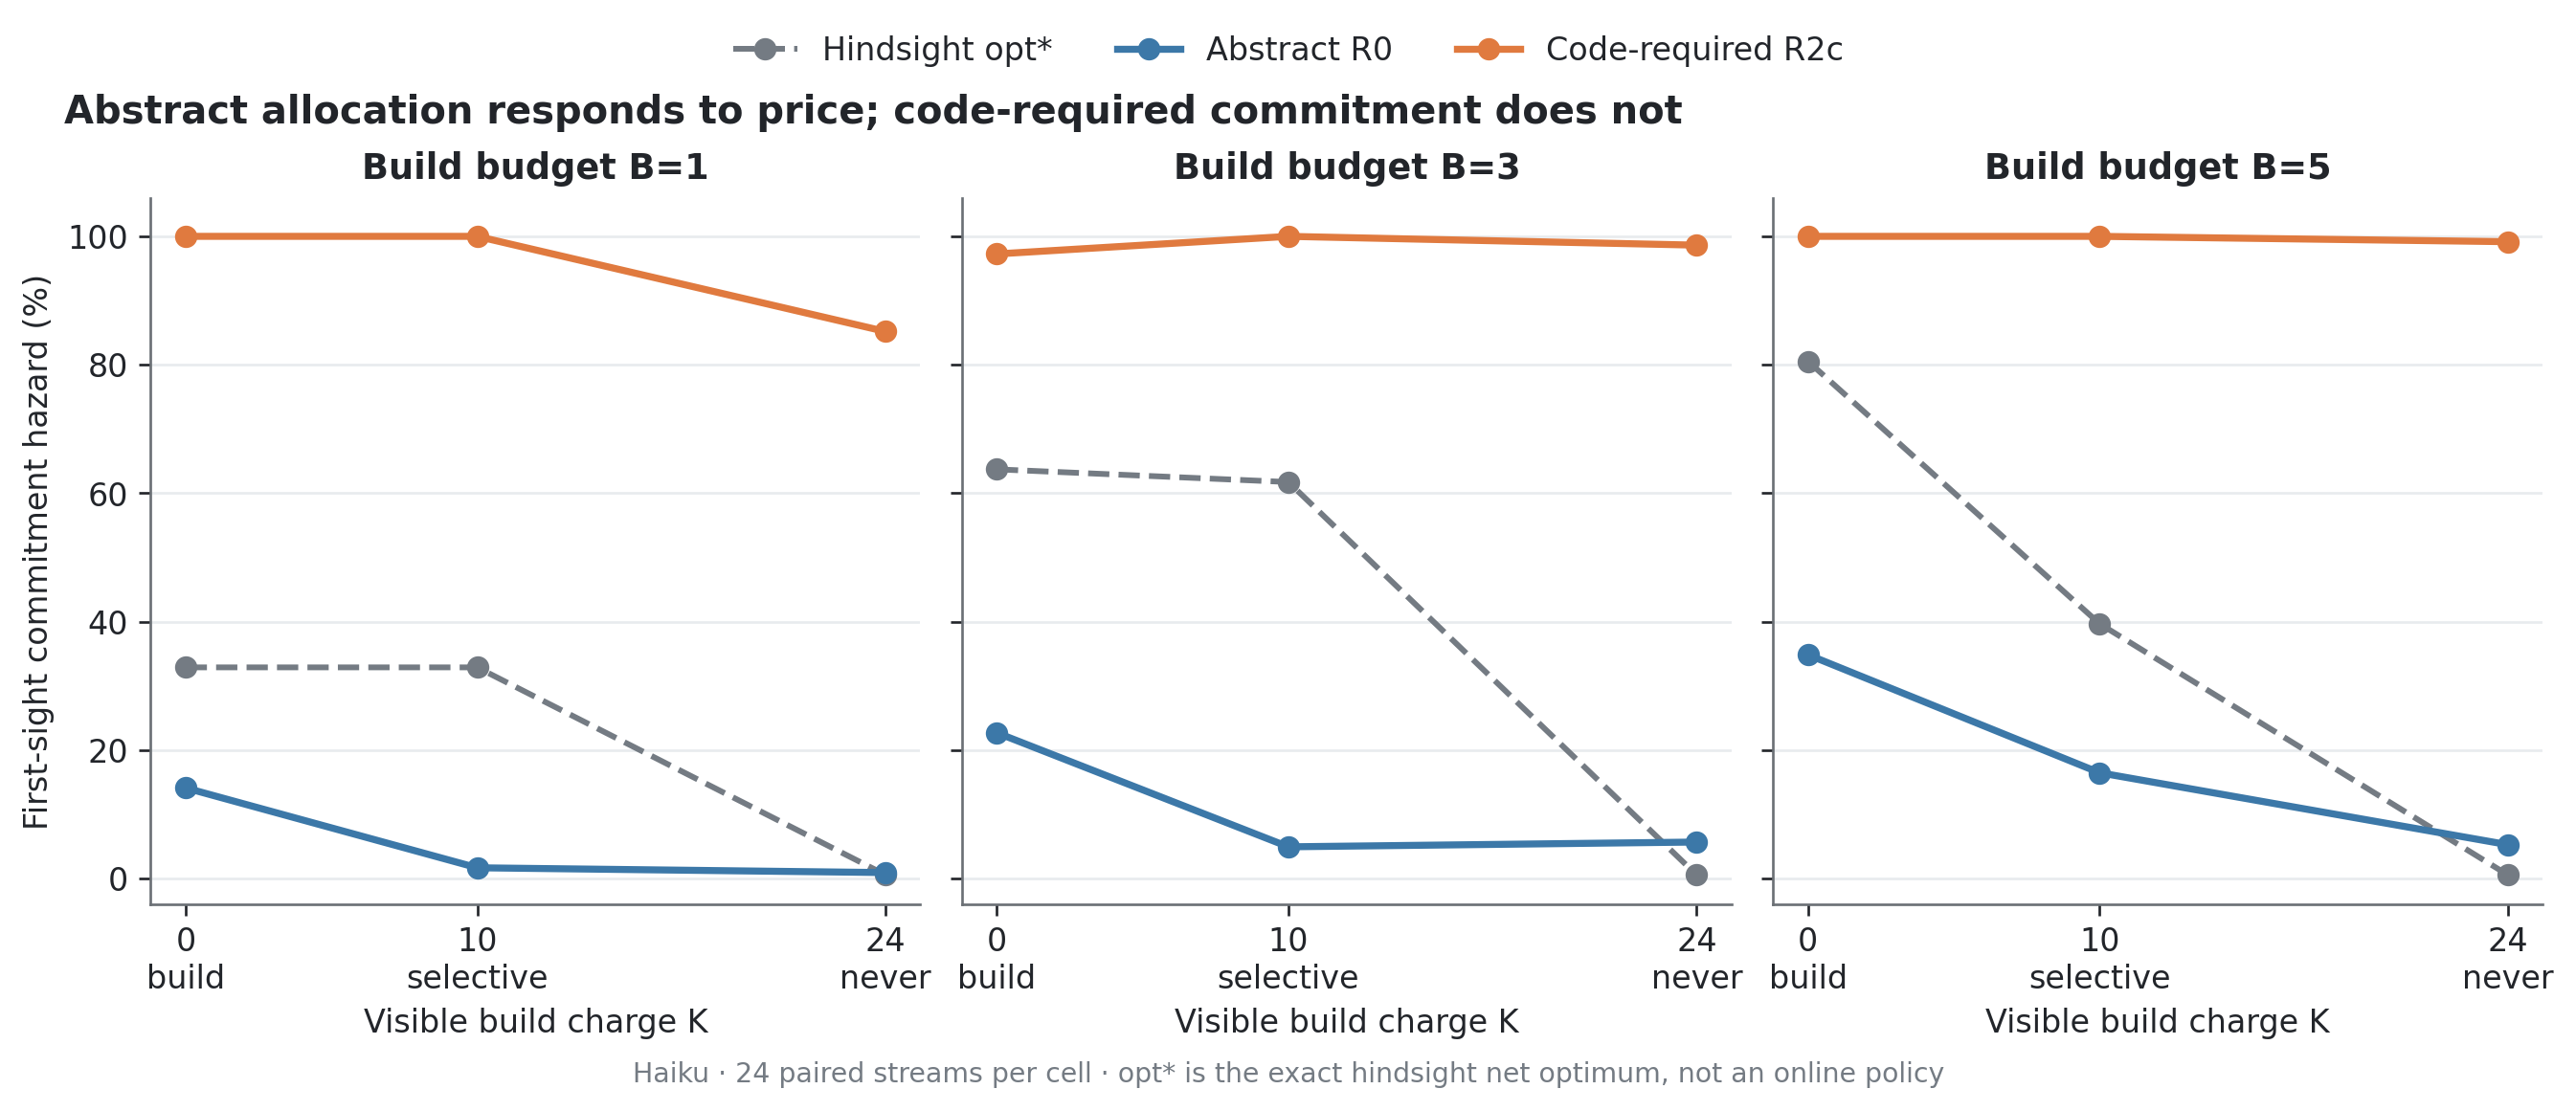
\includegraphics[width=\linewidth]{figs/fig3_economic_elasticity.png}
\caption{\textbf{Abstract allocation responds to price; code-required
commitment does not.} First-sight commitment hazard is shown across visible
build charges for each build budget. The abstract R0 policy becomes more
selective as construction grows expensive, broadly co-moving with the exact
hindsight net optimum. R2 remains near 100\% first sight, including at
$K=24$, where the hindsight optimum commits on only about 1\% of eligible
first-sight turns. Each cell reuses the same 24 paired
Haiku streams; the hindsight reference is an offline upper bound, not an
online policy.}
\label{fig:economic}
\end{figure}

\subsection{Convergent case study: acquisition without constructive activation}
\label{sec:qwen-case-study}

As a separate proof-of-possibility case study, we ask whether reward can install
reserve in a model that is initially eager in both frames, and whether the
learned policy then activates during script creation. Starting from untouched
Qwen2.5-Coder-14B-Instruct, one QLoRA \citep{dettmers2023qlora} per-decision PPO
\citep{schulman2017ppo} run with no demonstrations reduces first-sight
commitment on 24 held-out abstract streams from 74\% to 35\%; lateness rises
from 0.403 to 0.750, and collected items rise from 95\% to 102\% of the
Bayesian comparator. The critic receives true class-rate features unavailable
to the actor \citep{pinto2018asymmetric}. A second, independent PPO run under
the same recipe -- differing only in that its training rollouts disclose $N$,
where the first run's training predates the $N$-disclosure protocol --
reproduces acquisition more strongly still (first-sight
commitment 6\%, lateness 1.51, collecting par with the comparator), so
acquisition is replicated, though neither run demonstrates robust or
sample-efficient learning. Appendix~\ref{app:rl} gives the
training procedure and pilot history.

The learned reserve is not tied to the literal words \emph{ball},
\emph{color}, and \emph{bag}. On three unseen lexical reskins that preserve the
abstract keep/pass structure, RL-final makes 29\% of commitments on first sight,
versus 65\% for the base model, with mean lateness 0.838 versus 0.587. This is
lexical generalization, not general task transfer.

Transfer nevertheless remains context-bound. Under the class-bound-r3-v1
protocol (24 matched q8\_0 reusable-script streams, EFR4, write-budget slots
attributed to the hidden class they can execute on), RL-final and base make
94.3\% and 90.9\% of unique-class builds on first sight (50/53 and 50/55; mean
lateness 0.057 and 0.109). RL-final is not more reserved than base under this
corrected allocation unit -- if anything slightly less so, within noise at
$n=24$ -- reconfirming the no-transfer verdict after the R2 allocation-unit
repair. The second training run makes the same boundary starker: despite its
6\% abstract first-sight rate, it builds 95\% of its scripts at first sight
under the identical protocol (52/55, mean lateness 0.055). All three panels
are mechanically clean (zero malformed, unknown, or
refused tool calls across all 72 sessions).
Expressing the abstract reskins through zero-argument keep/pass tool calls
produces partial transfer, uniform across vocabularies (50\% for RL-final
versus 87\% for base). Thus the learned disposition survives new words but
degrades under a
modality change and is absent in reusable construction
(Figure~\ref{fig:rl-transfer}). Detailed modality probes, per-vocabulary
results, and retry diagnostics are deferred to Appendix~\ref{app:rl}.

\begin{figure}[t]
\centering
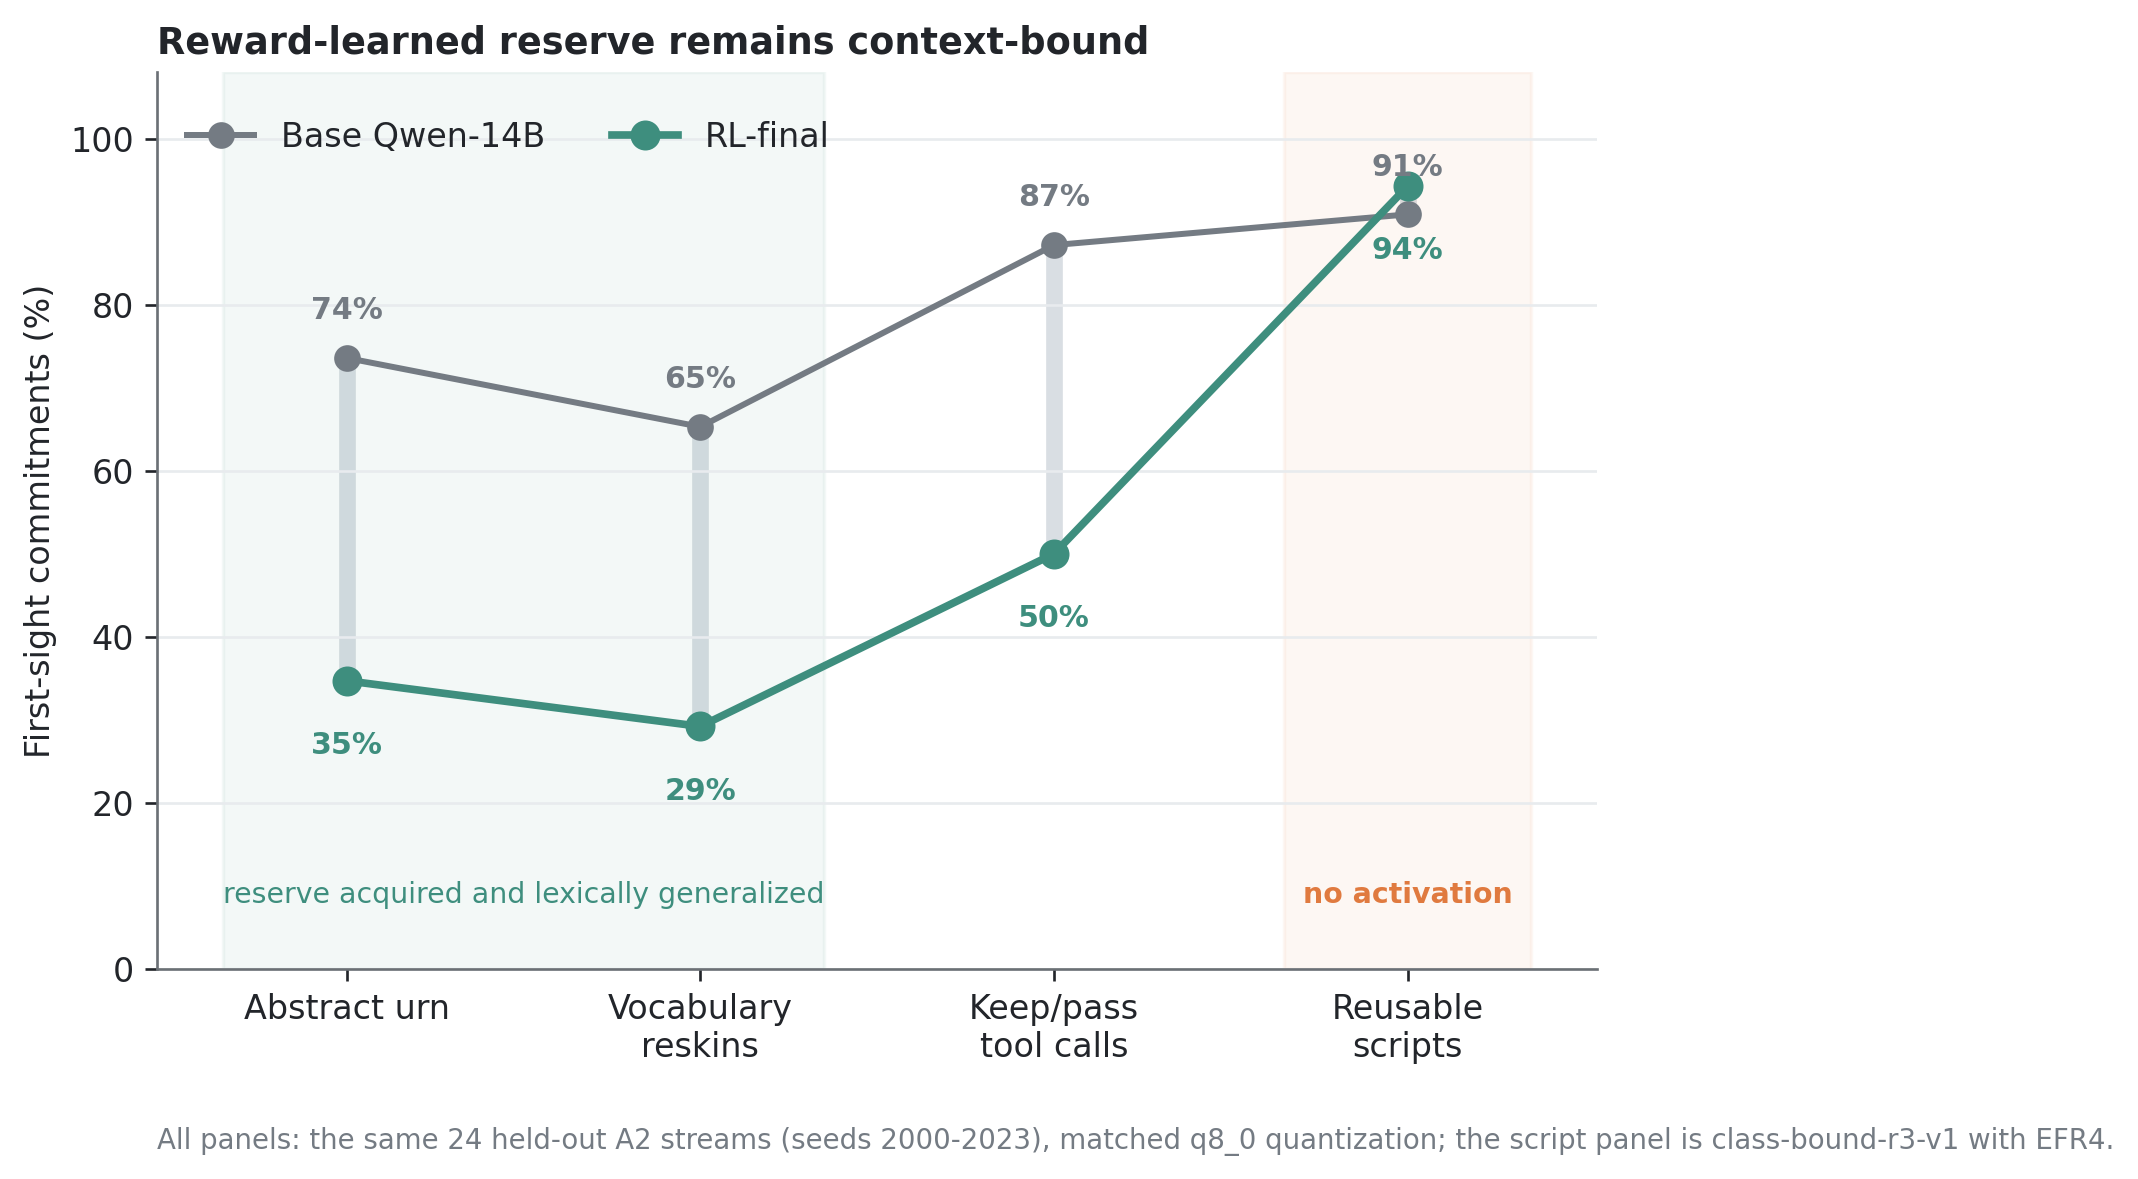
\includegraphics[width=0.82\linewidth]{figs/fig5_rl_transfer_boundary.png}
\caption{\textbf{Reward-learned reserve remains context-bound.} The trained
Qwen-14B policy reserves in the original abstract urn and across three lexical
reskins. Transfer weakens when the same keep/pass decision is expressed through
tool calls and disappears in reusable script construction, where base and
RL-final are 90.9\% and 94.3\% first sight -- RL-final is not the more reserved
of the two. All four columns come from one uniform evaluation protocol:
the same 24 held-out A2 streams (seeds 2000--2023), matched q8\_0
quantization, and (for the script column) class-bound-r3-v1 with EFR4.}
\label{fig:rl-transfer}
\end{figure}

The pooled first-sight rate summarizes an outcome; the decision rule behind it
is visible directly by conditioning P(KEEP) on how many times the current
color has already appeared in the stream (Figure~\ref{fig:reserve-policy}).
Base keeps at a roughly flat rate from the first sighting onward (58.2\%
at occurrence 1, 57.1\% at occurrence 2, 91 and 21 decisions respectively),
consistent with an eager policy that does not condition on recurrence. RL-final
inverts this at the two occurrences that carry most of the mass: it passes on
the first sighting (22.9\%, 25/109) and keeps once recurrence is confirmed on
the second (83.3\%, 40/48) -- a defer-then-confirm rule, not merely a lower
overall keep rate. The second training run sharpens the same rule (3.1\% at
occurrence 1, 60.0\% at occurrence 2). Occurrences three and beyond have small
per-bucket $n$ (2--8 decisions) and are not part of this claim.

\begin{figure}[t]
\centering
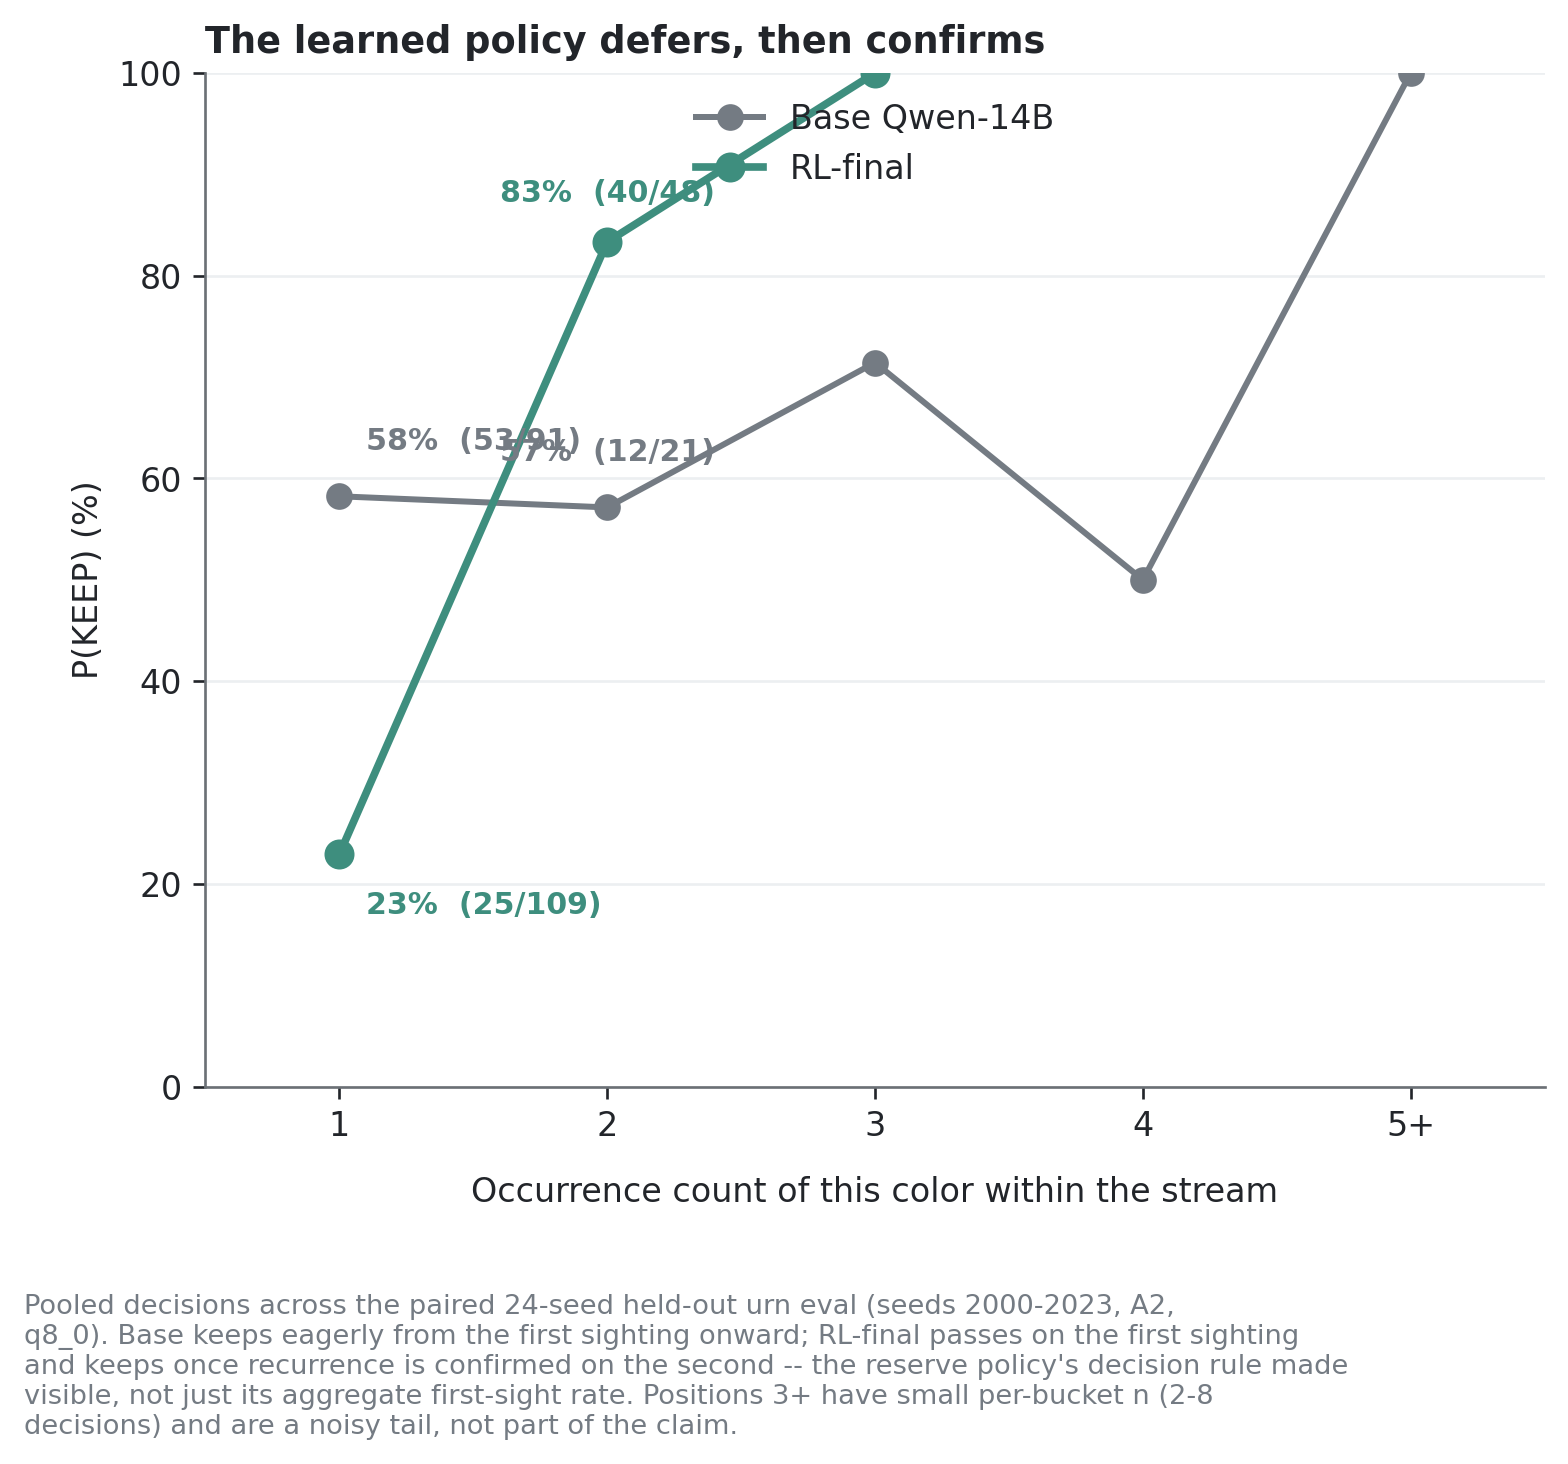
\includegraphics[width=0.82\linewidth]{figs/fig6_reserve_policy_shape.png}
\caption{\textbf{The learned policy defers, then confirms.} P(KEEP) pooled
over the paired 24-seed held-out urn eval (seeds 2000--2023, A2,
q8\_0), conditioned on how many times the current color has already appeared.
Base keeps eagerly from the first sighting onward. RL-final passes on the
first sighting and keeps once recurrence is confirmed on the second -- the
reserve policy's decision rule made visible, not just its aggregate
first-sight rate. Occurrences three and beyond have small per-bucket $n$ (2--8)
and are a noisy tail.}
\label{fig:reserve-policy}
\end{figure}

\section{Discussion}

\paragraph{Possession, acquisition, and activation.}
The experiments separate three questions that ordinary tool benchmarks
conflate. A policy may be absent, as in baseline Qwen; acquired from reward but
context-bound, as in the Qwen case study; or already present but suppressed by
constructive framing, as in every frontier model we test. At R3 the
``preserved'' cell of this taxonomy is empty: no tested model carries its
abstract allocation policy into full reusable-script construction. What the
panel measures instead is the \emph{depth} of the trigger -- code emission
alone suffices to suppress Haiku, Opus, and (in degenerate form)
GPT-5.4-mini, while GPT-5.6 Sol withstands R2 and collapses only at full
construction. That graded structure is the benchmark's diagnostic payoff: it
distinguishes how much constructive context a model's allocation policy
survives, even though none survives all of it.

\paragraph{Why might construction suppress allocation?}
Required code emission may invoke a reactive coding-assistant policy centered
on solving the visible instance. It may also collapse ``solve now'' and
``invest for later'' into one salient action. R2 rules out
correctness-dependent reward and hand-solving availability as necessary causes,
but it does not separate emission from the compliance and effort induced by an
instruction to produce correct code, nor does it identify a neural mechanism.
The transcript and code-quality evidence supports
current-instance fixation only as a bounded behavioral interpretation.

\paragraph{Implications for agents.}
Tool-building systems should separate the decision to invest from execution of
the build. An explicit recurrence ledger, remaining-budget state, or evidence
threshold could make the investment decision legible before code generation
begins. These are design implications, not tested interventions. Evaluation
should score delayed utility and library opportunity cost rather than only
immediate task success or tool correctness.

\paragraph{Implications for capability evaluation.}
A useful online-investment evaluation needs two conditions. An abstract
competence gate establishes that the model can reserve at all; the constructive
condition tests whether timing survives realistic action. Either alone is
ambiguous. Future work should test whether cross-frame preservation predicts
the quality of libraries and long-horizon resource allocation in naturalistic
repository, data-cleaning, API, and analysis workloads.

\section{Limitations}

The benchmark uses one synthetic numeric environment with engineered hot and
trap recurrence. Real tasks have ambiguous class boundaries, nonstationary
frequencies, partial reuse, and variable construction quality. R2 intentionally
decouples payoff from correctness to study a code-required claim condition; it
does not separate emission from compliance or output effort and is not a
realistic model of artifact value.

The core causal ladder is centered on Haiku and uses 24 independent canonical
streams (12 preregistered plus a 12-seed extension added post hoc under the
identical generator and harness). Hundreds of crossed sessions do not increase
the independent stream sample beyond 24. The model panel establishes that the
R3 failure recurs across two frontier families and one trained open-weight
policy, with heterogeneous failure modes; it does not establish a scaling
trend, a broad population estimate, or that untested models must fail. The
full economic response
surface is run only on Haiku, so GPT-5.6 Sol's R2 result shows comparative
selectivity under one paired condition, not cross-frame equivalence or economic
optimality at varying prices.

The Bayesian urn comparator is prior-dependent and mismatched to the engineered
generator. We therefore treat timing as primary and use the exact hindsight
net optimum only for realized economic regret. That optimum is unavailable to
an online model and should not be mistaken for an implementable policy.

The RL evidence contains two successful runs, both with a privileged critic;
the second run independently reproduces both the acquisition and the
transfer-failure results. Neither run demonstrates non-privileged
learnability or sample efficiency.
Finally, prompt and tool-choice formats affect deliberation. The framing ladder
is coarse rather than fully factorial: the R0-to-R1 step bundles the shift to a
tool-call claim action with the introduction of real problem content, so the
isolated trigger is established by the R1-to-R2 contrast (which holds content
fixed and adds only required code), not by R1 alone. Harness repairs were logged
transparently, but occurred during benchmark development.

\section{Conclusion}

Reusable tool creation is not only a coding problem; it is an online investment
decision under uncertain reuse. Paired experiments show that every model we
test -- across two frontier families and a reward-trained open-weight policy
-- demonstrates a recurrence-conditioned allocation policy in the abstract
frame and fails to express it under full reusable-script construction. The
failure modes differ: eager collapse, degenerate under-commitment, a
front-loaded and never-revisited opening batch. The trigger depth differs
too: required code emission alone suppresses Haiku, Opus, and GPT-5.4-mini,
while GPT-5.6 Sol's selectivity at that rung -- the panel's evidence that the
code-required task is passable -- gives way only at full construction. In
Haiku, the collapsed policy is also nearly invariant to visible economics,
and a Qwen reserve policy installed by reward, replicated across two
independent training runs, does not activate during construction. Online
tool allocation is therefore a real and measurable capability boundary at
current frontier scale, and agents that must invest well may need the
decision to build separated from the act of building.

\bibliography{allocation}

\appendix

\section{Reconstruction Details}
\label{app:reconstruction}

\subsection{Streams and session state}

All confirmatory Haiku, Opus, and GPT comparisons use canonical seeds
2000--2023 (the original 2000--2011 plus a 2012--2023 seed-extension panel
generated by the identical procedure and run under the identical harness). For each seed, a local pseudorandom generator first permutes the
eight procedure families
\texttt{lcg}, \texttt{modpow}, \texttt{continued\_frac},
\texttt{crt\_solve}, \texttt{josephus}, \texttt{quadratic\_map\_mod},
\texttt{xorshift\_steps}, and \texttt{matrix\_power\_mod} across three hot and
five trap roles. Hot classes jointly receive probability 0.85 and traps 0.15,
uniformly within role. The generator samples $T=60$ class identities
i.i.d. and rejection-samples until at least one trap occurs in the first $B$
positions ($B=3$ in the core comparison). Numeric instances are generated at
magnitude 100 for the canonical Haiku, GPT, and primary Opus R3 conditions. The
Opus R3 arm holds the complete latent stream fixed---family, class ID, role,
rate, realized count, occurrence position, and arrival order---and reuses the
same magnitude-100 numeric rendering as Haiku and both GPT models, so all four
models answer literally identical problem instances. It does not pin or
relocate any family. Structural projections match the canonical Opus urn
artifacts on 24/24 seeds. Class metadata are hidden; only rendered item or
problem text is shown to the model. Haiku R0, R1, R2, and R3 reuse the
same saved magnitude-100 stream for each seed. Appendix~\ref{app:magnitude-sensitivity}
separately reports a magnitude-1000 completeness check for Opus's R3 arm, the
pool used earlier in this project to foreclose Opus's partial hand-solving
ability.

Each commitment consumes one of $B$ slots and is irreversible. Subsequent
members of a committed class are automatically collected or solved and produce
no new decision. Sessions stop making decisions when the budget is exhausted,
but scoring includes all later members of committed classes. Economic sessions
use the same streams and cross $B\in\{1,3,5\}$ with
$K\in\{0,10,20,24\}$; $K$ changes only the disclosed one-time charge and net
score.

\subsection{Prompt and tool reconstruction}

The artifact retains every rendered user message, assistant response, tool
call, and generated stream. Exact prompt generators and schemas are in
\texttt{urn\_common.py}, \texttt{urn\_session.py},
\texttt{urn\_tool\_session.py}, \texttt{claim\_solver\_session.py},
\texttt{claim\_solver\_code\_session.py}, and
\texttt{session\_state.py}. To remove ambiguity about substitutions, the core
A2 prompts have $T=60$, $N=8$, and the current $B$ inserted into the following
templates.

\paragraph{R0 allocation instructions.}
The system states that 60 items are drawn one at a time; at any draw the model
may KEEP the current item or PASS; at most $B$ items may be kept; keeping an
item immediately collects it and every future item with the same visible
attribute; passing scores zero; already-kept attributes are auto-collected and
do not create another decision; and choices do not change the stream. The A2
disclosure is:
\begin{quote}\small
There are exactly 8 distinct colors in the bag, but you are not told which
colors are common or rare, nor how many balls of each color there are; you
learn the rates only from the draws you have seen.
\end{quote}
R0 ends with the exact response instruction
\begin{quote}\small
For each draw, think briefly (one or two sentences), then end your reply with
EXACTLY one line: \texttt{DECISION: KEEP} or
\texttt{DECISION: PASS}.
\end{quote}

\paragraph{R1/R2 allocation instructions.}
Both prompts state that 60 numeric problems arrive one at a time, each has a
hidden type, exactly eight types occur, rates are initially unknown, a solver
may be claimed at most $B$ times, a claim scores the current and all future
problems of that type, skipping scores zero, decisions are final, and the model
must call exactly one of \texttt{claim\_solver} or \texttt{skip\_solver}.
R1 explicitly says not to compute an answer and uses two zero-argument tools.
R2 instead adds the following exact requirement:
\begin{quote}\small
You must provide \texttt{code}: a real, correct Python function
\texttt{def solve(inputs: dict) -> float} that solves problems of this type---it
stands in for every future problem of the same type for the rest of the
session, so it should actually work, not just handle the problem currently
shown.
\end{quote}
The R2 \texttt{claim\_solver} schema therefore has one required string
property, \texttt{code}; \texttt{skip\_solver} remains a zero-argument object.
The prompt does not disclose that correctness is excluded from reward. For an
economic cell, both R0 and R2 add the exact statement that committing costs
$K$ points once, each collected or solved problem remains worth one point, and
declining costs nothing. R3 uses the reusable-script harness's
\texttt{write\_script}, \texttt{run\_script}, and answer tools; the complete
prompt and schema generators are in \texttt{driver.py} and
\texttt{session\_state.py}, and complete resulting transcripts are stored in
\path{runs/arm_a1_announce_n-announced/} for Haiku and
\path{runs/arm_a1_announce_opus_n-announced_canonical-structure/}
for the repaired Opus endpoint.

\subsection{Models and generation settings}

Claude runs use \texttt{claude-haiku-4-5-20251001} and
\texttt{claude-opus-4-8}. GPT runs use
\texttt{gpt-5.4-mini-2026-03-17} and \texttt{gpt-5.6-sol}. Provider-default
temperature is held fixed across paired arms. Claude R1 and R2 use
\texttt{tool\_choice=auto}; forcing a tool call suppressed deliberation in
calibration. GPT uses \texttt{reasoning\_effort=none} in both arms and
\texttt{tool\_choice=auto} for R2. Maximum output is 512 tokens for R0,
1500 for R1, 2500 for R2, and 4096 per R3 turn, with a 300,000-token session
cap. Opus R3 sessions stop immediately after the third successful script write;
all 24 terminate on budget exhaustion without hitting the token or per-seed
cost breaker, and contain no malformed or unknown calls. GPT-5.4-mini R3
sessions truncate on write-budget exhaustion when any script is written (6/24
seeds) and otherwise run to the 300,000-token session cap or full stream
completion (18/24 seeds); all 24 are mechanically clean, with zero malformed,
unknown, or refused tool calls. GPT-5.6 Sol R3 sessions likewise truncate on
budget exhaustion for 12/24 seeds and on the 300,000-token session cap for the
other 12; all 24 are mechanically clean. Qwen starts from
\texttt{Qwen/Qwen2.5-Coder-14B-Instruct}; matched final
tool evaluations use q8\_0 base and adapted models with an 8192-token context.

\subsection{Competence gate and mechanical validity}
\label{app:mech-validity}

A GPT model passes the locked abstract competence gate only if all 24 R0
sessions complete, it makes at least 2.5 commitments per seed, no more than
50\% of realized commitments are first-sight, and its mean collection reaches
90\% of the same-information Bayesian comparator. The preregistered
suppression replication additionally requires at least 80\% R2 first-sight
among commitments, a pooled R2--R0 increase of at least 30 points, and a
positive lower endpoint for the paired bootstrap interval.

Transport or provider exceptions receive at most two additional attempts with
linear 1.5-second backoff. Model-level failures---no decision, multiple
decisive calls, an unknown function, malformed arguments, or an unparsable
response---are not retried; they default to the non-commit action and remain
counted as unresolved. A ladder rung is invalid if unresolved decisions exceed
10\%. Response-model identity, stream hash, malformed and unknown calls,
termination reason, usage, and token-cap hits are checked separately from
behavior. Only a mechanical failure permits a replacement run. For the final
Qwen script evaluation, empty-fence retries are fixed at four in both arms and
all attempts remain logged.

\paragraph{Qwen R2 exceeds the 10\% threshold; we report it anyway, unfiltered.}
Both Qwen R2 arms exceed the panel's 10\% unresolved-decision threshold by a
wide margin: base-q8 resolves 186/347 decisions (46.4\% unresolved) and
RL-final resolves 146/402 (63.7\% unresolved), against zero malformed or
unknown calls for every other model in Table~\ref{tab:score}. This is the same
idle-tail empty-fence generation failure documented for this model family in
Section~\ref{sec:qwen-case-study} -- common to base and RL-final, not an
RL-training artifact -- and it survives the same \texttt{empty-fence-retry=4}
mitigation used for the final Qwen script evaluation above: the retry breaks
runaway repetition and lets most sessions still spend their full write budget
(22/24 base-q8 seeds, 17/24 RL-final seeds reach \texttt{budget\_exhausted}
with all 3 claims placed), but does not restore a clean channel. Rather than
invoke the mechanical-failure exception to drop or resample the affected
seeds, we report Score pooled over all 24 seeds for both arms, unresolved
decisions included, because the two arms fail at different rates (2/24
base-q8 seeds versus 7/24 RL-final seeds never place their third claim before
the stream ends): excluding a model's own failed seeds would remove more of
precisely the outcomes that scored worst for whichever arm fails more often,
manufacturing a base-vs-RL gap out of the exclusion rule itself rather than
out of behavior. The unfiltered numbers (Table~\ref{tab:score}: 61.2\% for
both arms, collected 729 and 730 of 1192) are therefore the conservative,
selection-bias-free comparison, at the cost of reflecting a genuine 14B
capability limitation on this harness's code-writing tool schema rather than
a fully clean channel. We disclose this explicitly as a departure from the
10\% rule rather than silently reporting a number the stated methodology
would otherwise call invalid.

\subsection{Bootstrap estimands}
\label{app:bootstrap}

For each paired comparison, first-sight among commitments is computed within
seed, the second-arm value minus the first-arm value is taken, and paired seeds
are sampled with replacement 10,000 times using bootstrap RNG seed 0. The
reported point estimate is the arithmetic mean of seed differences and the
interval is the percentile interval. A seed with no commitments has an
undefined among-commitments proportion and is omitted only from that
conditional estimand; it remains in commitment, zero-commit, hazard, and
utility summaries. Economic endpoint interactions are computed per seed as
\[
\{h_{R0}(0)-h_{R0}(24)\}
-\{h_{R2}(0)-h_{R2}(24)\},
\]
separately for each $B$, and then resampled by seed. No session within a seed
is treated as an independent replicate.

\section{Magnitude Sensitivity Check}
\label{app:magnitude-sensitivity}

The main text reports Opus's R3 arm at magnitude 100, matching Haiku and both
GPT models so that all four models in the panel answer literally the same
problem instances. This magnitude was not the arm originally used earlier in
this project: an initial calibration found that at magnitude 100, Opus hand-solves
roughly 25--38\% of problems in isolation (\texttt{josephus} alone at
essentially 100\%), so a magnitude-1000 rendering was adopted specifically to
foreclose that escape valve before the R3 timing result was trusted. We
include that magnitude-1000 arm here purely for completeness, not as the
primary result.

Rerunning the identical 24 canonical seeds, harness, and truncation protocol at
magnitude 1000, Opus makes 72/72 R3 builds at first sight (100\%) with zero
mean lateness; the R3-minus-R0 paired difference is $+95.8$ points, 95\%
seed-bootstrap interval $[+91.7,+100.0]$. This is statistically indistinguishable
from the magnitude-100 result reported in the main text (98.6\% first sight,
71/72 builds, mean lateness 0.014, paired difference $+94.4$ points
$[+88.9,+98.6]$): the two intervals overlap substantially, and neither timing
estimate is degenerate at $N=24$. Josephus accounts for seven of the 72 builds
in both arms, all at first sight in both, so its known hand-solvability at any
magnitude does not drive either result.

The magnitude change therefore has no detectable effect on Opus's
construction-time eagerness. We report the magnitude-100 arm as primary
because it removes an asymmetry across the model panel, not because the
magnitude-1000 arm turned out to be confounded: at magnitude 100, with a
genuine if narrow hand-solve alternative available on every turn, Opus
submitted a raw, script-free answer to an unbuilt class only once across the
full 24-seed panel, and that attempt was incorrect. Artifacts are in
\path{runs/arm_a1_announce_opus_n-announced_canonical-structure_mag100_class-bound-v1}
(magnitude 100, this appendix's comparison arm and the main text's primary
result) and
\path{runs/arm_a1_announce_opus_n-announced_canonical-structure_class-bound-v1}
(magnitude 1000, the completeness check).

\section{Complete Economic Summaries}
\label{app:economic}

Table~\ref{tab:econ-full} reports the principal behavioral and utility
quantities on the plotted charge surface, $N=24$ seeds (2000--2023). Hazard is pooled over eligible
first-sight turns; all other columns are means over the 24 seeds. Zero-commit
incidence is 0\% in every displayed cell.

\begin{table}[H]
\centering
\scriptsize
\caption{Economic surface with timing, commitment, and utility outcomes reported
together. Net is collected or solved items minus $K$ times commitments; regret
is against the exact hindsight net optimum.}
\label{tab:econ-full}
\resizebox{\linewidth}{!}{%
\begin{tabular}{llrrrrr}
\hline
Frame & $(B,K)$ & Hazard (\%) & Commits & Lateness & Net & Regret \\
\hline
R0 & $(1,0)$  & 14.1 & 1.00 & 1.42 & 10.6 & 8.9 \\
R0 & $(1,10)$ & 1.7  & 1.00 & 3.21 & 3.1 & 6.4 \\
R0 & $(1,24)$ & 0.9  & 1.00 & 3.00 & -10.5 & 10.6 \\
R0 & $(3,0)$  & 22.7 & 3.00 & 1.21 & 37.5 & 12.1 \\
R0 & $(3,10)$ & 4.9  & 3.00 & 2.29 & 10.1 & 9.6 \\
R0 & $(3,24)$ & 5.7  & 2.96 & 2.21 & -33.4 & 33.5 \\
R0 & $(5,0)$  & 34.8 & 4.83 & 0.83 & 51.0 & 4.9 \\
R0 & $(5,10)$ & 16.5 & 4.67 & 1.39 & 1.6 & 18.1 \\
R0 & $(5,24)$ & 5.3  & 4.33 & 2.45 & -61.8 & 61.8 \\
\hline
R2 & $(1,0)$  & 100.0 & 1.00 & 0.00 & 10.0 & 9.5 \\
R2 & $(1,10)$ & 100.0 & 1.00 & 0.00 & 0.0 & 9.5 \\
R2 & $(1,24)$ & 85.2 & 1.00 & 0.08 & -14.1 & 14.2 \\
R2 & $(3,0)$  & 97.3 & 3.00 & 0.03 & 32.7 & 17.0 \\
R2 & $(3,10)$ & 100.0 & 3.00 & 0.00 & 2.9 & 16.8 \\
R2 & $(3,24)$ & 98.6 & 3.00 & 0.00 & -38.5 & 38.6 \\
R2 & $(5,0)$  & 100.0 & 5.00 & 0.00 & 51.5 & 4.4 \\
R2 & $(5,10)$ & 100.0 & 5.00 & 0.00 & 1.5 & 18.2 \\
R2 & $(5,24)$ & 99.2 & 5.00 & 0.01 & -68.5 & 68.6 \\
\hline
\end{tabular}%
}
\end{table}

\section{Reward-Learning Details}
\label{app:rl}

Both analyzed runs use QLoRA and per-decision PPO for 20 outer steps,
25 fresh training seeds per step, four rollouts per seed, one epoch per update,
learning rate $6\times10^{-5}$, and rollout temperature 1.2. Training seeds
begin at 9000 and do not overlap evaluation seeds. The critic observes the
actor's ordinary state plus true class-rate features; the actor never receives
those rates. Exact Monte Carlo returns are used without discounting. No
demonstrations enter training. The runs differ in one respect: the first run's
training rollouts predate the $N$-disclosure protocol and do not disclose
$N$; the second run's training rollouts disclose $N$, matching the A2
evaluation condition. Both runs' step-0 credit-assignment gates pass
(positive mean advantage for hot-class keeps and trap passes, negative for
trap keeps and first-sight hot passes), and both produce monotone reserve
acquisition over training.

Each unchanged final checkpoint is evaluated on the original ball vocabulary
and on treasure-chest/coin/crest, quiver/arrow/feather, and
cauldron/potion/label reskins. All retain $N=8,T=60,B=3$, the same latent
streams, disclosed $N$, and free-text keep/pass decisions. A second probe
changes only the
decision channel to required zero-argument keep/pass calls. Tool-call
transfer is uniform across vocabularies (49--51\% first sight for RL-final
versus 83--93\% for base); an earlier probe panel had shown strong
vocabulary sensitivity, which did not reproduce under the final
quantization-matched A2 protocol. The final reusable-script comparison uses 24
paired seeds
2000--2023 under the class-bound-r3-v1 protocol, matched q8\_0 quantization,
calibrated script success, and four empty-fence retries in both base and
RL-final arms; write-budget slots are attributed to the hidden class they can
execute on, repairing the allocation-unit mismatch with R2. Both arms are
mechanically clean (zero malformed, unknown, or refused tool calls across all
48 sessions); the base arm truncates on write-budget exhaustion for 20/24
seeds and the 300,000-token session cap for the remaining 4/24, while
RL-final truncates on budget exhaustion for 23/24 and the token cap for 1/24.
The second run's script arm, run under the identical protocol, is likewise
mechanically clean (zero refused tool calls across its 24 sessions).

\section{Commands and Artifact Manifest}

The core runs are reproduced from the repository root with the $N=24$
seed-extension panel (2000--2023); the original preregistered panel used
\texttt{\$(seq 2000 2011)} in place of \texttt{\$(seq 2000 2023)} below.
{\scriptsize
\begin{verbatim}
PYTHONPATH=. python -u -m scripts.creator.tool_disposition_benchmark.urn_session \
  --model haiku --announce-n --seeds $(seq 2000 2023)
PYTHONPATH=. python -u -m scripts.creator.tool_disposition_benchmark.urn_tool_session \
  --model haiku --announce-n --seeds $(seq 2000 2023)
PYTHONPATH=. python -u -m scripts.creator.tool_disposition_benchmark.claim_solver_session \
  --model haiku --announce-n --seeds $(seq 2000 2023)
PYTHONPATH=. python -u -m scripts.creator.tool_disposition_benchmark.claim_solver_code_session \
  --model haiku --announce-n --seeds $(seq 2000 2023)
PYTHONPATH=. python -u -m scripts.creator.tool_disposition_benchmark.arm_a1_announce \
  --model haiku --announce-n --full-stream --seeds $(seq 2000 2023) --cap 20.0 --unit-cap 2.0
PYTHONPATH=. python -u -m scripts.creator.tool_disposition_benchmark.arm_a1_announce \
  --model opus --announce-n --canonical-structure --magnitude 100 --publication \
  --seeds $(seq 2000 2023) --cap 3.0 --unit-cap 0.75
PYTHONPATH=. python -u -m scripts.creator.tool_disposition_benchmark.run_economic_surface \
  --seeds $(seq 2000 2023)
PYTHONPATH=. python -u -m scripts.creator.tool_disposition_benchmark.analyze_economic_surface \
  --seeds $(seq 2000 2023) --charges 0 10 20 24
\end{verbatim}
}
Core artifacts are
\path{runs/urn_haiku_n-announced},
\path{runs/urn_tool_haiku_n-announced},
\path{runs/claim_solver_haiku_n-announced},
\path{runs/claim_solver_code_haiku_n-announced},
\path{runs/arm_a1_announce_n-announced}, and
\path{runs/economic_surface_haiku}. The primary Opus R3 artifact (magnitude
100) is
\path{runs/arm_a1_announce_opus_n-announced_canonical-structure_mag100_class-bound-v1};
the magnitude-1000 completeness check (Appendix~\ref{app:magnitude-sensitivity})
is
\path{runs/arm_a1_announce_opus_n-announced_canonical-structure_class-bound-v1}.
GPT artifacts are under
\path{runs/economic_surface_gpt-5.4-mini-2026-03-17} and
\path{runs/economic_surface_gpt-5.6-sol}; each contains the exact model
identifier, settings, stream, transcript, usage, and per-seed analysis.

\section{Transcript Excerpts}
\label{app:transcripts}

This appendix collects verbatim model rationales behind the qualitative claim in
Section~\ref{sec:gate}: abstract (R0) decisions reason prospectively about
recurrence and budget, whereas full-construction (R3) decisions center on the
instance in front of the model, register budget only near exhaustion, and reuse
scripts reactively. All excerpts are quoted verbatim (ellipses mark elision) and
are drawn from the same models and canonical streams (seeds 2000--2023) reported
in the main text. Provenance is given as run directory and seed; per-seed
transcripts contain the full turn-by-turn context.

\paragraph{R0: prospective reserve and confirmation on recurrence.}
In the abstract urn frame, commitments are deferred explicitly to gather
frequency evidence and are triggered only once a type's rate is established.
\begin{itemize}
  \item Haiku, \path{runs/urn_haiku_n-announced}, seed 2000, third draw
  (\textsc{pass}): ``I've seen three different colors in three draws (red, blue,
  green). With 60 draws total and 8 colors in the bag, I still need more
  information about the frequency distribution. Passing to gather more data is
  the right strategy at this early stage.''
  \item Opus, \path{runs/urn_opus_n-announced}, seed 2000, second draw
  (\textsc{pass}): ``Still gathering information; too early to commit a keep.''
  \item Opus, \path{runs/urn_opus_n-announced}, seed 2000, seventh draw
  (\textsc{keep}, third occurrence of the type): ``Red has now appeared 3 times
  in 7 draws --- a strong rate. With 53 draws left, keeping red should yield
  many more.''
\end{itemize}

\paragraph{R3: instance-focused construction, late budget awareness, reactive reuse.}
In the full-construction frame the same models write a script for the problem
currently on screen. Budget is mentioned only when nearly gone, and reuse is
considered only after a type recurs rather than reserved for in advance.
\begin{itemize}
  \item Opus,
  \path{runs/arm_a1_announce_opus_n-announced_canonical-structure_mag100_class-bound-v1},
  seed 2000, problem 1 (first write, no budget reasoning): ``I'll write a script
  for this bit-manipulation problem type.''
  \item Opus (same run), seed 2008, first write: ``I'll write a CRT solver
  script since this type may recur.'' Then, on its third and last write: ``I
  have 1 write left. Let me use it for this LCG type which may recur.'' --- the
  first mention of the write budget in the session arrives only as it is
  exhausted.
  \item GPT-5.4-mini,
  \path{runs/arm_a1_announce_gpt-5.4-mini-2026-03-17_n-announced_write-budget-v2_class-bound-v1},
  seed 2000, reuse decision: ``I can reuse the existing script only if the hidden
  type matches; here I'll just calculate directly since it's simple.''
\end{itemize}

GPT-5.6 Sol is omitted from the excerpts above because its R3 sessions emit no
visible deliberation text (its snapshot runs at
\texttt{reasoning\_effort=none}); its construction decisions are observable only
through the tool-call sequence, which shows the same front-loaded, first-sight
pattern.

\end{document}